\documentclass[journal]{IEEEtran}
\usepackage{graphicx}
\usepackage{booktabs}
\usepackage{array}
\usepackage{url}
\usepackage{cite}
\usepackage{amsmath,amssymb}
\usepackage{balance}
\begin{document}

\title{Machine learning in battery management systems: a structured scoping review and classification of 103 peer-reviewed studies, 2019--2026}

\author{Hussain~Touhid~Siddiquee,~Syeda~Salsabil~Islam~Ariya,~and~Jasimul~Islam~Chowdhury%
\thanks{Manuscript received September 2026. (Corresponding author: Hussain Touhid Siddiquee.)}%
\thanks{The authors are with Leading University, Sylhet, Bangladesh. The classified corpus,
the conference sensitivity set, and the complete analysis pipeline are publicly available at
\texttt{github.com/touhidsiddiqueeraj-bit}.}}

\markboth{IEEE Transactions Submission, September 2026}{Siddiquee et al.: Machine Learning in Battery Management Systems}

\maketitle

\begin{abstract}
Machine learning (ML) has moved from a promising addition to battery research to a load-bearing component of modern battery management systems (BMS). This paper presents a structured scoping review of 103 peer-reviewed journal articles published between 2019 and 2026 that apply machine learning to battery management tasks, assembled from a Crossref-verified pool of peer-reviewed journal articles and classified uniformly by management function, method family, chemistry, data source, and validation practice. The corpus is classified by management function (state of charge, state of health, remaining useful life, charging control, thermal management, fault and safety, and cross-cutting themes), by method family, by battery chemistry, by data source, and by validation practice. The bibliometric analysis reveals a clear five-year evolution. Classical shallow learners such as Gaussian process regression and support vector machines dominated the early window, contributing 11 of the 23 corpus papers published from 2019 through 2021, with deep recurrent architectures rising sharply in 2022--2023. From 2022 onward, physics-informed and hybrid model--data approaches became one of the fastest-growing families, reaching 24 of 103 corpus papers, while optimization-augmented learning and transfer learning together account for a further 16 papers. The first large-language-model-based battery management studies appear in 2025--2026. Health estimation and prognostics remain the largest application cluster (35 papers), followed by the cross-cutting cluster (24), state estimation (17), fault and safety (9), charging control (8), and thermal management (8). Three structural weaknesses persist across the five-year window. First, validation practice is heterogeneous and often weak: only 9 of 103 studies demonstrate their estimators on real vehicle or fleet data, while 17 rely on within-cell or k-fold splits that overstate generalization. Second, benchmark-data dependence is high but narrow; the Severson/Toyota, NASA, and CALCE datasets recur across ostensibly independent studies, inflating apparent comparability. Third, the laboratory-to-field gap remains the field's defining challenge: sub-percent accuracy claims rarely survive chemistry, temperature, and current-profile shifts, and onboard compute constraints are discussed in a minority of works. The review's sharpest finding is that physics-informed architectures, often assumed to improve reliability by construction, are validated less rigorously than purely data-driven peers (54\% versus 73\% strong-protocol share): physics priors reduce data demand but do not substitute for rigorous out-of-distribution testing. The review closes with a research agenda prioritizing cross-domain validation standards, uncertainty-aware and interpretable models, edge-deployable architectures, and the safe integration of foundation models into safety-critical BMS software.
\end{abstract}

\begin{IEEEkeywords}
machine learning, battery management systems, lithium-ion batteries, state of charge, state of health, remaining useful life, deep learning, physics-informed neural networks, transfer learning, battery safety
\end{IEEEkeywords}

\section{Introduction}

\subsection{Electrification and the battery management problem}

Lithium-ion batteries now anchor three converging transitions: the electrification of road transport, the proliferation of stationary storage in renewable-heavy grids, and the electrification of aerospace, marine, and industrial systems. In each of these settings, the battery is not a passive component but an actively managed asset whose usable capacity, lifetime, and safety depend on operating decisions made in real time. The battery management system is the embedded cyber-physical layer that makes those decisions: it senses cell voltages, currents, and temperatures; estimates unobservable internal states; protects against over-charge, over-discharge, and thermal abuse; balances cells; and increasingly negotiates charging strategies with the surrounding power system \cite{r1}.

The difficulty of the management problem stems from the fact that the quantities that matter most --- state of charge (SOC), state of health (SOH), internal temperature, and the onset of degradation or fault mechanisms --- are not directly measurable. They must be inferred from noisy, partially observable terminal measurements under widely varying operating conditions. Model-based approaches built on equivalent-circuit or electrochemical models have served the industry well, but they face a persistent trade-off between fidelity and computational tractability, and their parameters drift as cells age \cite{r2}. It is in this inference-and-decision layer that machine learning has made its most forceful entry.

\subsection{The rise of machine learning in battery management}

Machine learning entered battery management through estimation. Early applications treated SOC and SOH estimation as supervised regression on hand-engineered features, using support vector machines, Gaussian process regression, and shallow neural networks. Two studies then reset expectations for the whole field. Severson and colleagues showed that the entire cycle life of a lithium-ion cell could be predicted with a median test error near 9\% using only features extracted from the first hundred cycles, on a public dataset of 124 cells \cite{r3}. Attia and colleagues demonstrated closed-loop Bayesian optimization of fast-charging protocols, identifying high-quality protocols in 2.5 months rather than the 18 months typical of manual experimentation \cite{r4}. Together these results reframed battery management as a data problem in which learning systems could outperform hand-tuned models both in estimation accuracy and in experiment efficiency.

The five years that followed produced a wave of published applications across every BMS function: recurrent and convolutional networks for SOC and SOH \cite{r5}\cite{r6}, graph and transformer architectures for prognostics \cite{r7}\cite{r8}, physics-informed neural networks that embed electrochemical and thermal priors into learning systems \cite{r9}\cite{r10}, transfer learning schemes that port estimators across chemistries and vehicles \cite{r11}\cite{r12}, reinforcement learning agents for charging and prognostic model selection \cite{r13}, and, most recently, large language model (LLM) agents for fleet-scale risk analysis and vehicle-cloud battery management \cite{r14}\cite{r15}.

\subsection{Existing reviews and the literature gap}

The review literature has grown alongside the applications, but it is fragmented along the same axes as the primary studies. Function-specific reviews cover SOC estimation \cite{r16}\cite{r17}, SOH estimation \cite{r18}, and prognostics \cite{r19} in depth, while method-specific reviews follow individual threads such as deep-learning state estimation \cite{r20}, physics-informed learning for impedance-based diagnostics \cite{r21}, or interpretable ML for prognosis \cite{r22}. Domain-anchored reviews examine fault diagnosis and safety \cite{r23}\cite{r24} and thermal management \cite{r25}, alongside broader degradation-method surveys \cite{r26}. What is largely missing is a cross-functional, quantitative account of the field's trajectory: which method families are actually being used for which management tasks, on which data, validated how, and how that picture has shifted over the last five years.

This gap matters because the field's self-image drives its research allocation. If, for example, most published health estimators are validated on within-cell splits of public datasets, the community's sense of progress is calibrated to a benchmark regime that differs sharply from fleet deployment. If interpretability claims are concentrated in a small method family, the safety case for certification-grade ML in production BMS is weaker than the volume of publications suggests. Answering such questions requires a corpus-level, cross-functional account of the field rather than another narrative synthesis of one function.

\subsection{Contribution of this paper}

This paper makes four contributions. First, it assembles a verified corpus of 103 peer-reviewed journal articles (2019--2026) on machine learning for battery management, in which every reference's bibliographic metadata was confirmed against the Crossref registry by direct DOI resolution. Second, it develops a two-axis classification framework --- BMS function $\times$ method family --- extended with chemistry, data-source, and validation-practice fields, and applies it uniformly to all 103 papers. Third, it quantifies the field's five-year evolution across functions, methods, data, and validation (Section 3), identifying the shift from classical learners through deep sequence models to physics-informed hybrids, optimization-augmented learning, and early foundation-model applications. Fourth, it provides a critical, function-by-function review of what the corpus actually demonstrates (Sections 4--8) and distills a gap-driven research agenda (Section 9).

Fig. 1 previews the analysis, mapping the entire corpus across management functions and method families: the field's center of gravity sits squarely in the health-prognostics complex, hybrid model--data approaches now span every function, and learning-based charging control remains a concentrated Bayesian-optimization stronghold. The remainder of the paper is organized as follows. Section 2 details the review methodology: search strategy, screening procedure, inclusion and exclusion criteria, and the classification framework, together with its limitations. Section 3 presents the corpus overview and five-year bibliometric analysis. Sections 4 through 7 review machine learning for state estimation, health estimation and prognostics, charging control, and thermal management, fault detection, and safety, respectively. Section 8 examines cross-cutting directions --- physics-informed learning, interpretability and uncertainty, digital twins and cloud BMS, and foundation models. Section 9 formulates research gaps and future directions, and Section 10 concludes.

\begin{figure*}[!t]
\caption{The corpus mapped across battery-management functions and method families (91 primary-application papers; see Section 2.5 for terminology). Cell values are paper counts. The 12 corpus reviews are excluded here; the ``of which reviews'' column of Table 3 states the reconciliation directly, and no excluded review belongs to the physics-informed family, so that column's corpus total of 24 (Table 2) is unchanged.}
\centering
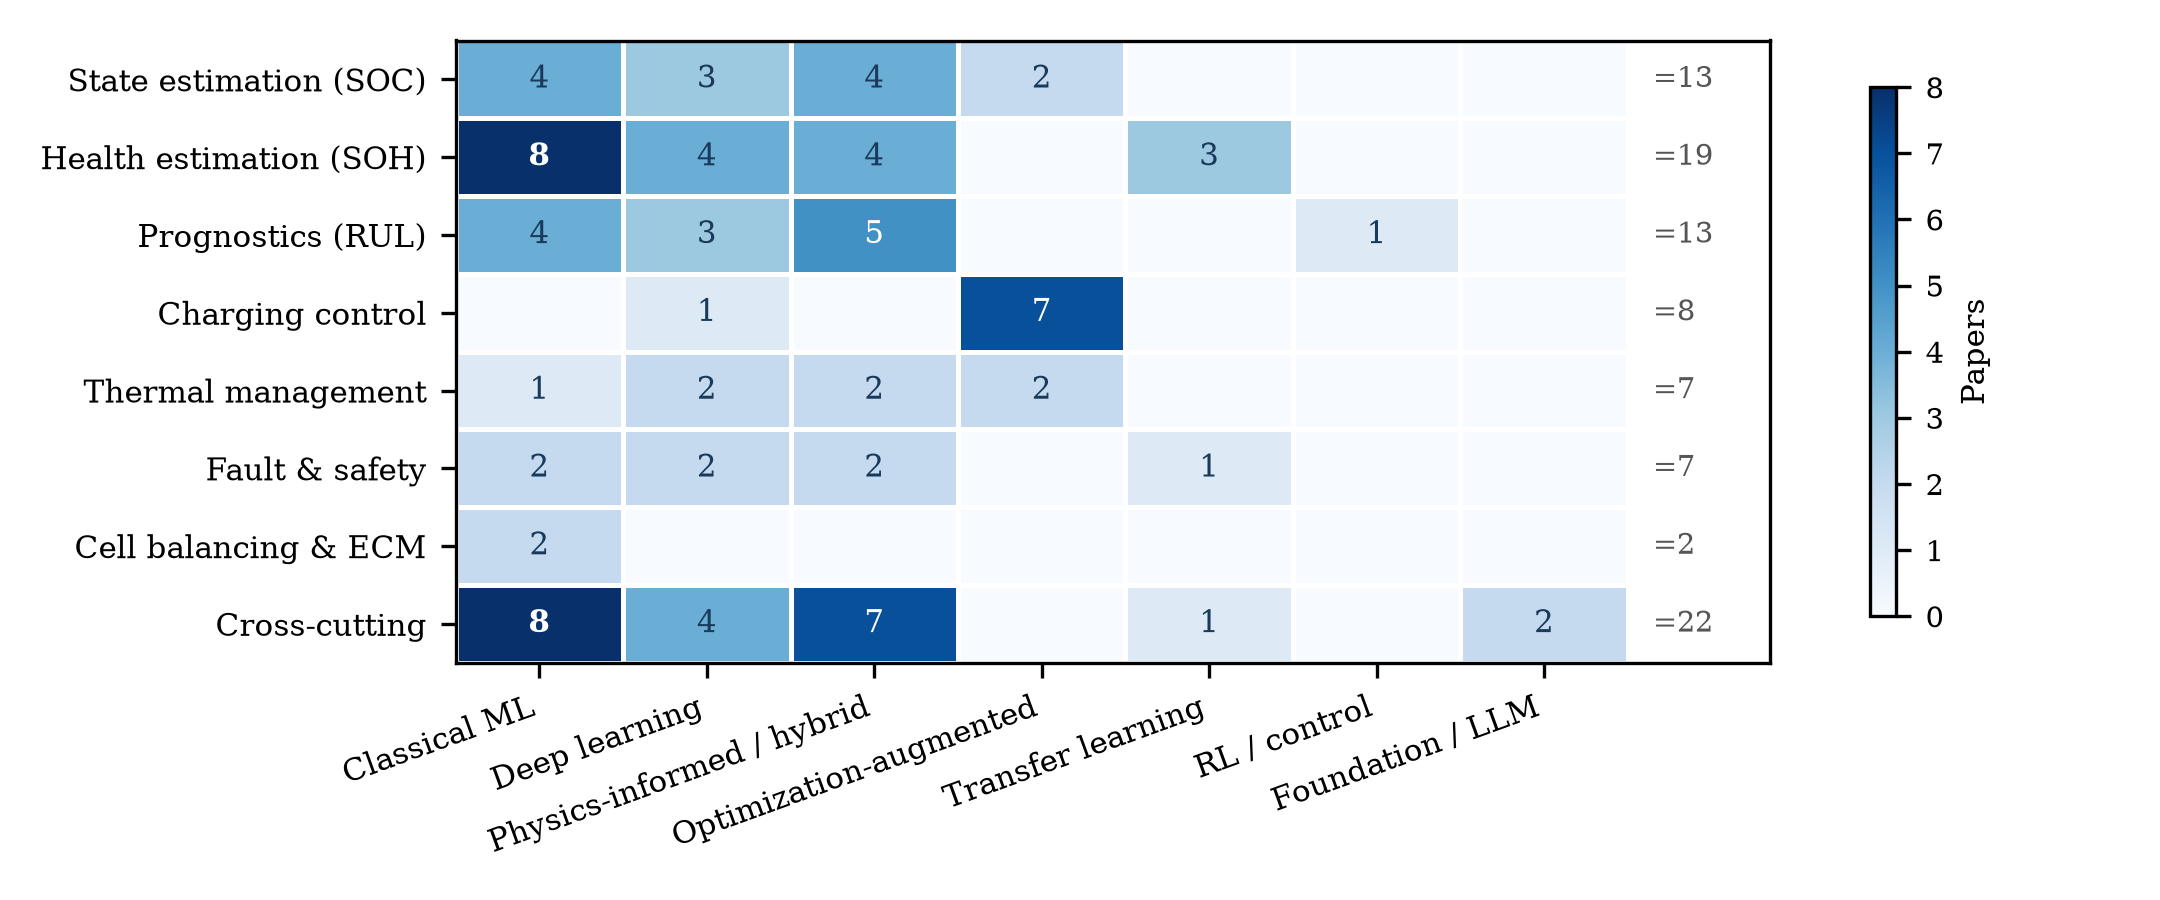
\includegraphics[width=6.9in]{figs/fig1_function_method_map.png}
\label{fig:fig1_function_method_map.png}
\end{figure*}

\section{Review Methodology}

\subsection{Scope and objective}

The objective of this review is to characterize the current state and recent evolution of machine learning applied to battery management, understood as the set of estimation, protection, and control functions performed by or in support of a battery management system. The scope covers SOC estimation, SOH estimation and capacity tracking, remaining useful life (RUL) prediction and early-life prognosis, charging strategy optimization, thermal-state estimation and battery thermal management, fault diagnosis, anomaly detection and safety prediction, and cross-cutting methodological themes (physics-informed learning, transfer learning, interpretability, digital twins, cloud and fleet management, and foundation models). Battery \textit{design} and \textit{materials-discovery} applications of machine learning fall outside the scope except where they directly support a management function, such as manufacturing-quality prediction of cell capacity.

\subsection{Literature search strategy}

All candidate records were retrieved programmatically from the Crossref REST API between 4 and 5 September 2026 using 30 bibliographic query strings spanning the application areas listed above (for example, ``state of charge estimation lithium-ion battery machine learning'', ``remaining useful life prediction battery deep learning'', ``physics-informed neural network lithium-ion battery'', and ``large language model battery''). Queries were issued in four passes: a top-cited pass over 2020--2026 sorted by citation count; a relevance-sorted recency pass restricted to mid-2024 onward; and two dedicated relevance-sorted passes restricted to 2020--2022 and to 2023, which together yielded 3,000 retrieved records. After DOI-based deduplication --- 1,450 duplicates removed --- 1,550 unique records remained. Six landmark studies --- including the early-life prediction study \cite{r3} and the prognostics review \cite{r2} --- were additionally safeguarded as forced seeds: five were retrieved and verified individually because citation-sorted retrieval had crowded them out, and one was already among the top-cited hits.

Two properties of this search design should be stated plainly. First, the Crossref registry is a metadata registry, not a discovery engine of the kind Scopus or Web of Science provide; it was chosen deliberately, because the aim of this review is that every included record be individually verifiable by direct DOI resolution, which registry-native retrieval guarantees and secondary databases cannot. The cost is a recall floor: coverage depends on Crossref registration, and the usual cross-database triangulation is absent. Second, the top-cited pass inherits the biases of citation counts --- it favors established, English-language, high-profile work and mechanically over-weights older publications. The three remaining passes exist to counter exactly these biases, and all trend statements in this paper are statements about trends within this citation-weighted, English-language, journal-article sample rather than about the field in the aggregate.

\subsection{Screening and selection procedure}

The screening funnel is shown in Fig. 2. From 1,550 deduplicated records, a title-level relevance gate requiring both battery-related and machine-learning-related terminology retained 883 records and excluded 667 (predominantly adjacent-field papers --- general machine-learning methods, adjacent-domain bibliometrics, and battery electrochemistry without a learning component --- that surfaced through loose bibliographic matching). Venue and document-type screening then removed 84 records --- conference abstracts and proceedings series (e.g., ECS Meeting Abstracts, IET/IFAC proceedings), preprint servers (SSRN), and non-scholarly venues --- in line with the decision to restrict the corpus to peer-reviewed journal articles, leaving 799 eligible records. A function-quota selection step then drew 107 candidate articles from these, balancing the eight management functions and publication years; six landmark seed studies were confirmed or injected at this point (one already captured by the searches, five retrieved individually), giving 113 candidate articles. Full-text curation excluded 19 records --- corrigenda, misindexed records, scope mismatches (for example, vehicle-level lifecycle assessment or charging-infrastructure demand modeling without a BMS function), and quota-driven trimming of over-represented function clusters --- while 15 targeted additions were made from the screened pool for under-represented themes, a net change of $-$4 that yields the final corpus of 103 studies.

\begin{figure*}[!t]
\caption{Study-selection flowchart. Records were retrieved from the Crossref REST API on 4--5 September 2026, deduplicated, screened at title level for battery and machine-learning relevance, screened at venue and document-type level, and curated to the final 103-study corpus. Every included record's metadata was verified by direct DOI resolution against the Crossref registry.}
\centering
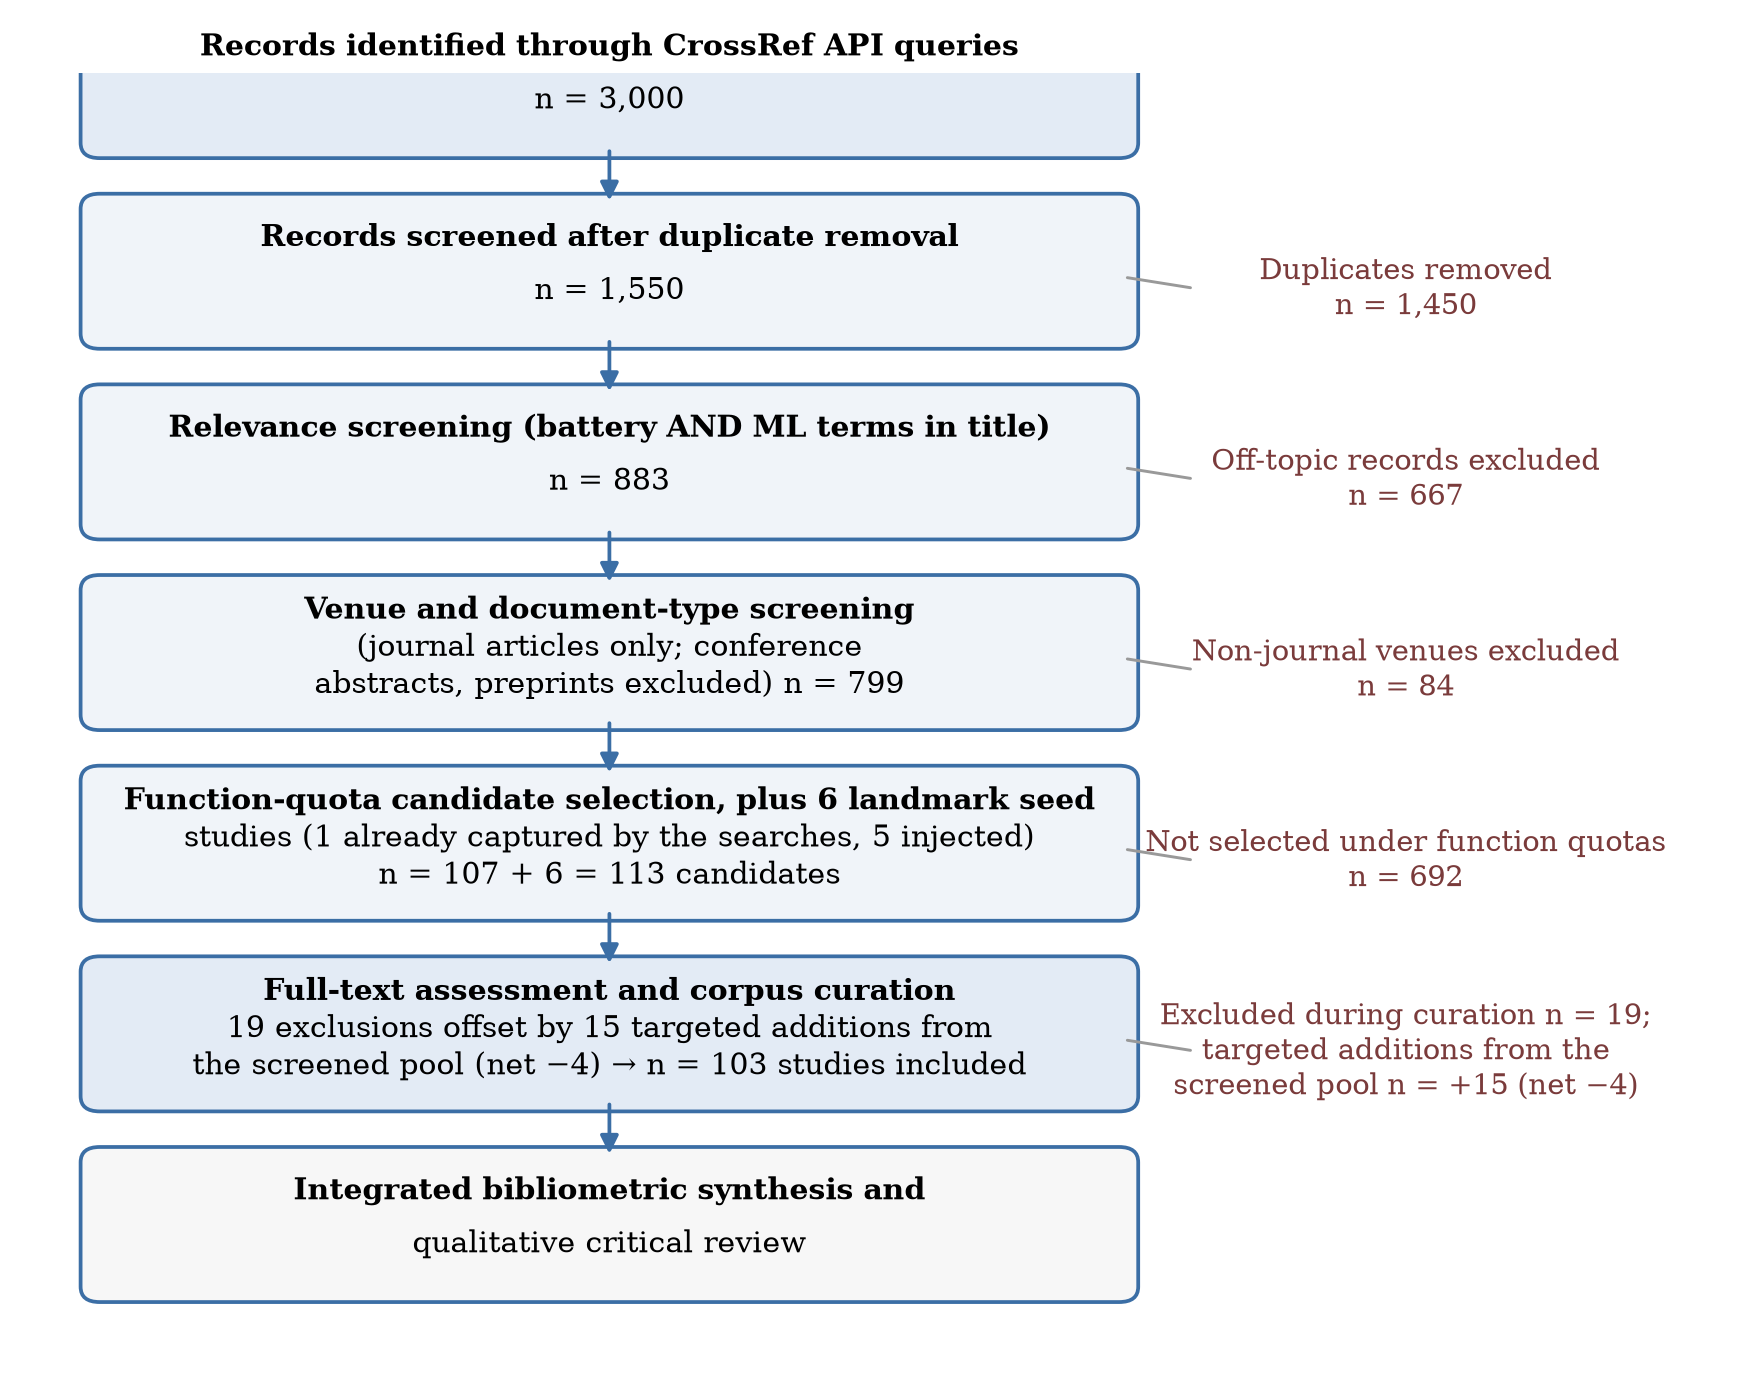
\includegraphics[width=5.9in]{figs/fig2_prisma.png}
\label{fig:fig2_prisma.png}
\end{figure*}

\subsection{Inclusion and exclusion criteria}

Table 1 summarizes the criteria. Inclusion required: (i) a peer-reviewed journal article; (ii) a battery or battery-system subject; (iii) machine learning as a substantive component of the contribution, whether estimation, control, diagnosis, or analysis; (iv) a publication year between 2019 and 2026, with 2019 admitted only for the field-defining early-life prediction study; and (v) English language. Exclusion criteria were: review-only papers without a primary application (admitted only into the cross-cutting cluster, capped at 12 studies), pure materials-discovery or cell-design papers, charging-infrastructure or grid-demand studies without an onboard management function, preprints and conference records, and duplicate-venue or misindexed records.

\begin{table*}[!t]
\caption{Inclusion and exclusion criteria applied during corpus screening}
\label{tab:table1}
\centering
\footnotesize
\begin{tabular}{|p{0.52in}|p{2.90in}|p{3.22in}|}
\hline
\textbf{Dimension} & \textbf{Included} & \textbf{Excluded} \\
\hline
Document type & Peer-reviewed journal articles & Conference abstracts/proceedings, preprints (SSRN), corrigenda \\
Subject & Batteries and battery systems with a management function & Materials discovery, cell design, grid/infrastructure demand modeling without BMS function \\
Method & ML as a substantive component (estimation, control, diagnosis, analysis) & Papers without a learning component \\
Period & 2020--2026 (plus one 2019 field-defining seed) & Pre-2020 publications \\
Verification & Metadata confirmed by direct Crossref DOI resolution & Unresolvable or mismatched records \\
Language & English & Non-English \\
\hline
\end{tabular}
\end{table*}

\subsection{Classification framework}

Each corpus paper was classified along six fields: (1) \textit{management function}, with eight values --- state estimation (SOC), health estimation (SOH), prognostics (RUL), charging control, thermal management, fault and safety, cell balancing and equivalent-circuit modeling, and a cross-cutting cluster for methodological and system-level themes; (2) \textit{method family}, with values including classical ML (Gaussian process regression, support vector machines, random forests, shallow networks), deep learning (recurrent, convolutional, attention and graph architectures), physics-informed and hybrid model--data learning, optimization-augmented learning (Bayesian optimization, surrogate-assisted and meta-heuristic schemes), reinforcement and control learning, transfer and domain adaptation, and foundation models/LLMs; (3) \textit{chemistry} (NMC, LFP, LCO, lithium-metal, lithium--sulfur, mixed, or unspecified); (4) \textit{primary data source} (own laboratory cycling, public datasets, laboratory impedance spectroscopy, real vehicle or fleet data, simulation, or multiple sources); (5) \textit{validation approach} (within-cell splits, cross-cell holdout, cross-chemistry or cross-domain transfer protocols, online/real-vehicle demonstration, experimental hardware, or simulation); and (6) a short coded summary of the headline finding and the principal limitation. Classification was performed by the lead author from registry-verified titles and abstracts, with conservative coding: where a paper's specifics could not be established confidently, broader categories were assigned. Three terms are used consistently hereafter: a \textit{corpus paper} is any of the 103 included studies; a \textit{primary study} (or \textit{primary-application paper}) is one of the 91 whose contribution is a primary application rather than a review; and the 12 reviews are identified by the method-family field and are excluded from Fig. 1. Papers are assigned a single dominant value per field even where several apply. A co-author verification pass reviewed all 103 classifications, but because it was corrective rather than an independent blind double-coding, we report it as a checking pass and claim no inter-rater agreement statistic; the counts in Section 3 should accordingly be read as one documented coding of the corpus rather than as ground truth. The complete classified dataset is released with this paper precisely so that independent coders can check, correct, or extend it --- and so that a formal reliability measurement can be run on the released labels.

\subsection{Comparative synthesis approach}

The synthesis proceeds on two tracks. Quantitatively, the classification fields are aggregated into cross-tabulations --- function by year, method family by year, chemistry, data source, and validation practice --- that characterize the corpus as a sample of the field's recent output (Section 3); every figure and every count in Section 3 was generated programmatically from the released dataset rather than compiled by hand; the full pipeline is publicly available in the repository accompanying this paper. Qualitatively, the review synthesizes each function's literature critically: what each cluster of methods assumes, what it demonstrates, and where its evidentiary support is thin (Sections 4--8). Cross-referencing the two tracks then yields the gap analysis of Section 9.

The methodology has limitations that readers should weigh. The corpus is drawn from Crossref-registered journal articles and therefore inherits that registry's coverage: influential conference papers (a significant venue for control-oriented BMS work) are excluded by design, and very recent articles registered with incomplete metadata may evade relevance screening. Title-level relevance screening can miss relevant papers whose titles avoid standard terminology, and citation-count ranking privileges English-language, high-profile venues. The classification fields were assigned by a single coder; no inter-rater reliability statistic is available. These limitations qualify the quantitative aggregates of Section 3, which should be read as a structured sample of the field's output rather than a census --- and they are the reason this paper describes itself as a scoping review with bibliometric classification rather than as a meta-analysis.

\section{Corpus Overview and Five-Year Evolution}

\subsection{Publication trend}

The corpus spans 2019--2026 with a strongly increasing and then broadening profile: 9 papers in 2020, 13 in 2021, 13 in 2022, 22 in 2023, 20 in 2024, 18 in 2025, and 7 in the first half of 2026, plus the 2019 seed (Fig. 3). Two caveats apply to any reading of this trend. First, the corpus is a curated sample, not a census: it preferentially captures highly cited and recent work, so the shape of the curve partly reflects curation choices as well as field growth. Second, citation counts mechanically over-weight older publications; age-normalized, the post-2023 output is larger than the raw counts suggest. With those caveats, the profile is consistent with the field's bibliometric explosion after 2019--2020 and with a maturing phase in which incremental single-function estimators increasingly compete with cross-cutting system-level contributions.

Citation weight tells a complementary story about influence. Citation counts throughout this paper are the Crossref registry's is-referenced-by-count values retrieved on 5 September 2026 and are included per paper in the released dataset; they are typically lower than Google Scholar counts for the same paper and should be compared only against themselves. The corpus accumulates roughly 18,400 recorded citations, but the distribution is steeply skewed: the median paper has 65 citations, while the 2019 seed alone holds 3,002 and the two 2020 landmark studies (Battery Lifetime Prognostics \cite{r2} and closed-loop fast charging \cite{r4}) hold 1,239 and 1,078 respectively. Median citations fall monotonically with publication year --- from 441 (2020) through 141 (2022) and 46 (2024) to single digits for 2026 publications --- which is partly an age effect and partly evidence that the field's attention concentrates on a small set of canonical results. For a scoping review this skew matters: narrative reviews that emphasize highly cited work systematically describe the field as it stood in 2020--2021, whereas the recent relevance-sorted portions of this corpus capture the current working frontier that citations have not yet caught up with.

\begin{figure}[!t]
\caption{Corpus composition by publication year (bars, left axis) with cumulative total (line, right axis). The 2019 seed study is included in the cumulative count.}
\centering
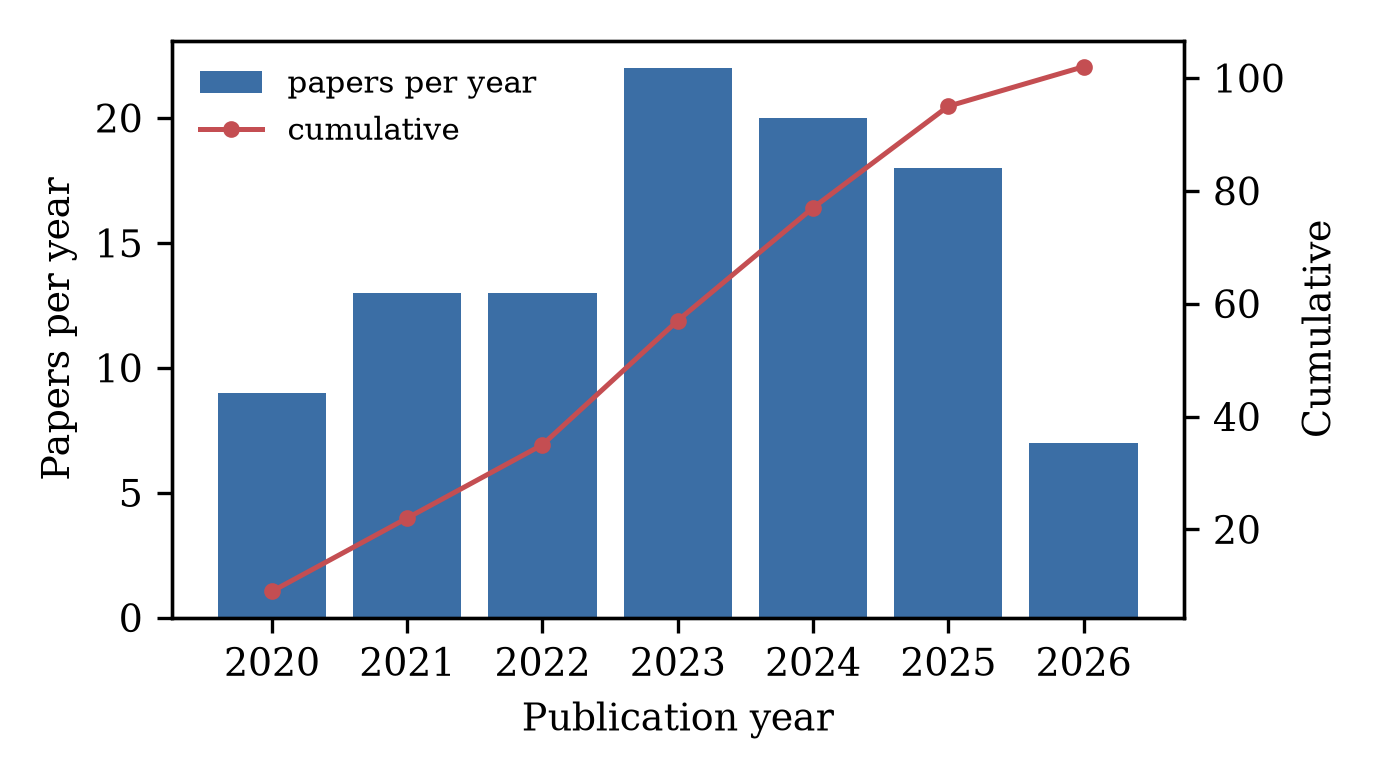
\includegraphics[width=\columnwidth]{figs/fig2_year_trend.png}
\label{fig:fig2_year_trend.png}
\end{figure}

\subsection{Method-family evolution}

The defining meta-finding of this review is the compositional shift in method families over the five-year window (Fig. 4, Table 2). Classical ML --- Gaussian process regression, support vector machines, ensemble regressors, and shallow networks on engineered features --- dominates the early corpus: 11 of the 23 papers published from 2019 through 2021. Deep sequence models (LSTM, GRU, CNN, attention and graph architectures) rise through 2022--2023 and remain the largest single family for prediction tasks thereafter. Physics-informed and hybrid model--data learning --- including physics-informed neural networks (PINNs), physics-constrained autoencoders, filter-embedded networks, and multiphysics-ML fusion --- emerges in 2021--2022, grows steadily, and becomes the modal family by 2024--2026: counted year by year, the family contributes 1 paper in 2020, 2 in 2021, 3 in 2022, 4 in 2023, 5 in 2024, 4 in 2025, and 5 in 2026 --- 14 of its 24 corpus papers fall in 2024--2026, and it is the largest single component of the 7 papers published in 2026 (Table 2 gives the corpus-wide totals; Fig. 4 the yearly shares). Optimization-augmented learning (Bayesian optimization for protocol design, surrogate-assisted multi-objective schemes, and meta-heuristic-tuned networks) peaks in 2023--2024 (11 papers). Transfer and domain-adaptation approaches appear consistently from 2022 and accelerate in 2024--2025 (5 papers), reinforcement learning remains scarce but visible (1 corpus paper), and the first foundation-model and LLM-based studies appear in 2025--2026 (2 papers) \cite{r14}\cite{r15}.

\begin{table*}[!t]
\caption{Method families in the corpus: representative techniques, strengths, and limitations}
\label{tab:TABLE_METH}
\centering
\footnotesize
\begin{tabular}{|p{0.81in}|p{0.37in}|p{2.03in}|p{1.62in}|p{1.57in}|}
\hline
\textbf{Method family} & \textbf{Papers} & \textbf{Representative techniques} & \textbf{Strengths} & \textbf{Limitations} \\
\hline
Classical ML & 29 & Gaussian process regression, SVM/SVR, ensembles, shallow networks on engineered features & Calibrated uncertainty; small-data friendly; cheap to embed & Feature engineering is manual; ceilings under complex dynamics \\
Deep learning & 19 & LSTM/GRU, CNN, attention/Transformer, autoencoders, graph networks & Learns features from raw curves; strong trajectory modeling & Data-hungry; weak extrapolation; opaque \\
Physics-informed / hybrid & 24 & PINNs, physics-constrained autoencoders, filter-embedded networks, multiphysics fusion & Structure aids extrapolation; reduced data demand & Inherits simplified-model bias; harder to train \\
Optimization-augmented & 11 & Bayesian optimization, surrogate-assisted multi-objective design, meta-heuristic-tuned networks & Sample-efficient protocol discovery; explicit trade-off handling & Offline tuning cost; surrogate bias \\
Transfer / domain adaptation & 5 & Domain-adversarial training, fine-tuning across chemistry/protocol & Directly targets the generalization gap & Negative transfer; needs shared protocols \\
Reinforcement / control learning & 1 & Deep-RL prognostic model selection & Adaptive decision-making along trajectories & Training stability; scarce hardware validation \\
Foundation models / LLM & 2 & Domain-tuned LLM agents for risk analysis and orchestration & Reasoning over heterogeneous text/system context & Hallucination risk; latency and cost \\
Review / perspective & 12 & Narrative and systematic syntheses & Maps the field; identifies shared gaps & No primary validation \\
\hline
\end{tabular}
\end{table*}

Within-family dynamics deserve comment. The persistent classical-ML share is not inertia: Gaussian process regression survives because it natively returns calibrated uncertainty --- the one property certification-minded applications cannot do without --- and because feature-based estimators remain the cheapest to embed. The deep-learning share consolidated around recurrent and attention architectures for trajectory data and convolutional architectures for curve data, with graph networks appearing where cell-to-cell or feature-to-feature relations matter. The optimization-augmented family grew along two distinct branches: meta-heuristically tuned networks (PSO, GA, and swarm variants), which improve accuracy at a documented training cost, and Bayesian or surrogate-assisted optimization of \textit{operating protocols}, which changes what can be experimentally discovered rather than merely what can be predicted. Conflating these two branches, as broad-brush surveys tend to do, obscures the more consequential of the two developments.

\begin{figure*}[!t]
\caption{Evolution of method-family shares in the corpus by publication year (share of papers published in each year). The 2019 seed (classical ML) is omitted for scale; families with fewer than two papers are pooled into their nearest parent family.}
\centering
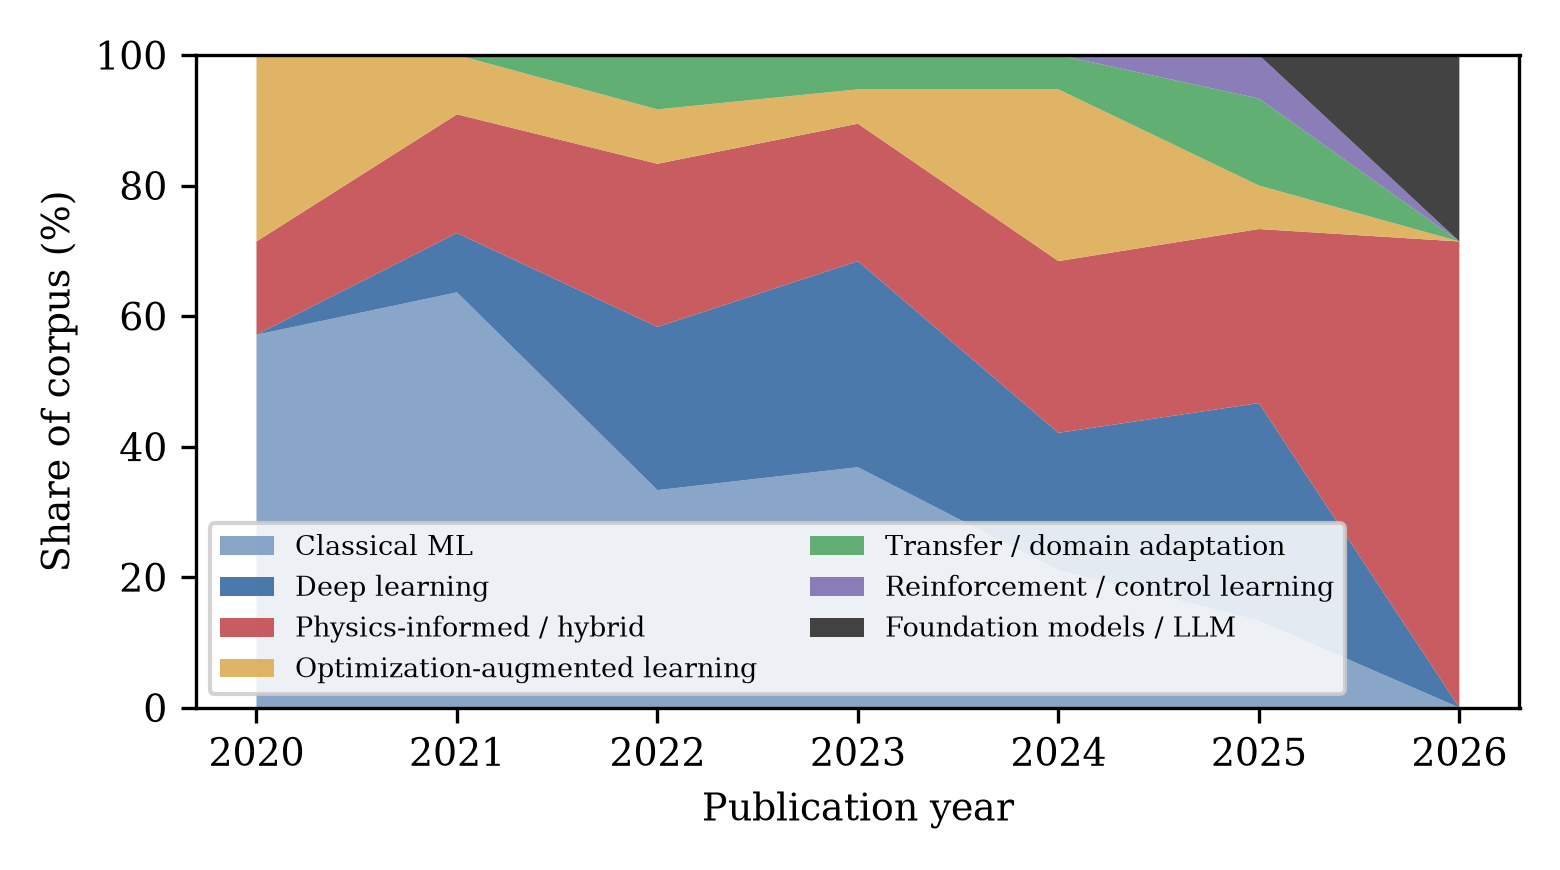
\includegraphics[width=5.0in]{figs/fig3_method_evolution.png}
\label{fig:fig3_method_evolution.png}
\end{figure*}

Three observations qualify this trajectory. First, the families are not mutually exclusive in practice --- a PSO-tuned LSTM is simultaneously deep learning and optimization-augmented learning --- and the corpus classification assigns each paper to its dominant family; the composition therefore understates method mixing. Second, the rise of physics-informed learning is partly a response to the recognized brittleness of purely data-driven models under distribution shift, but physics-informed papers in the corpus are, on average, validated no more stringently than others --- if anything somewhat less stringently, a point quantified in Section 3.4. Third, the foundation-model cluster is too small to represent a trend; its significance is that LLM-based management (fleet risk analysis and vehicle-cloud orchestration) is appearing in mainstream energy journals at all.

\subsection{Application-area distribution}

Functionally, the corpus is dominated by the health-prognostics complex: health estimation (20 papers) and remaining-useful-life prognostics (15) together account for 34\% of the 103-paper corpus, followed by the cross-cutting cluster (24, including reviews, physics-informed methods, interpretability, transfer learning, digital twins, cloud/fleet themes, and foundation models), state estimation (17), fault and safety (9), charging control (8), thermal management (8), and cell balancing/ECM (2) (Fig. 4). Fig. 5 matches the all-corpus totals of Table 3 (103 papers); Fig. 1, by contrast, is drawn over the 91-paper primary-application corpus and excludes the 12 reviews, with the per-function reconciliation stated in that figure's caption and in Table 3's ``of which reviews'' column. The concentration on SOH/RUL mirrors publication-volume patterns in the wider literature and reflects the strong commercial pull of lifetime prediction for warranties and second-life markets. By contrast, the thin representation of cell balancing is telling: balancing remains dominated by classical control practice, and ML has so far contributed mainly at the level of pack-level insight rather than as a balancing controller --- the corpus's most-cited balancing-related result is the demonstration that routine balancing can be dispensed with in well-managed packs, reducing hazardous lithium-plating side reactions \cite{r27}.

\begin{table*}[!t]
\caption{Corpus composition: management function by publication year. The Reviews column counts the 12 method-family reviews; Primary = Total $-$ Reviews gives the primary-application counts used in Fig. 1.}
\label{tab:TABLE2}
\centering
\footnotesize
\begin{tabular}{|p{1.64in}|p{0.32in}|p{0.32in}|p{0.32in}|p{0.32in}|p{0.32in}|p{0.32in}|p{0.32in}|p{0.32in}|p{0.36in}|p{0.50in}|p{0.50in}|}
\hline
\textbf{Function} & \textbf{'19} & \textbf{'20} & \textbf{'21} & \textbf{'22} & \textbf{'23} & \textbf{'24} & \textbf{'25} & \textbf{'26} & \textbf{Total} & \textbf{Reviews} & \textbf{Primary} \\
\hline
Cell balancing \& ECM & 0 & 0 & 0 & 0 & 1 & 1 & 0 & 0 & 2 & 0 & 2 \\
Charging control & 0 & 2 & 0 & 0 & 2 & 3 & 1 & 0 & 8 & 0 & 8 \\
Cross-cutting & 0 & 1 & 0 & 6 & 8 & 3 & 2 & 4 & 24 & 2 & 22 \\
Fault \& safety & 0 & 0 & 2 & 0 & 2 & 3 & 2 & 0 & 9 & 2 & 7 \\
Health estimation (SOH) & 0 & 2 & 3 & 2 & 4 & 3 & 4 & 2 & 20 & 1 & 19 \\
Prognostics (RUL) & 1 & 1 & 3 & 2 & 1 & 1 & 6 & 0 & 15 & 2 & 13 \\
State estimation (SOC) & 0 & 3 & 4 & 2 & 1 & 5 & 2 & 0 & 17 & 4 & 13 \\
Thermal management & 0 & 0 & 1 & 1 & 3 & 1 & 1 & 1 & 8 & 1 & 7 \\
Total & 1 & 9 & 13 & 13 & 22 & 20 & 18 & 7 & 103 & 12 & 91 \\
\hline
\hline
\end{tabular}
\end{table*}

Chemistry and venue concentration complete the corpus profile. NMC-type cells anchor 53 of the 103 studies and LFP 15; the remainder split across LCO, lithium-metal, lithium--sulfur, mixed panels, and unspecified chemistries --- a distribution that mirrors EV market share but leaves sodium-ion, solid-state, and high-temperature systems nearly absent from the ML-management literature. Venue concentration is equally marked: the Journal of Energy Storage (14 papers), Energy (13), and Applied Energy (9) head the corpus, with Journal of Power Sources, Energy Storage Materials, and Reliability Engineering \& System Safety following; IEEE transactions account for most of the remainder. The implication for readers is that the ML-BMS literature's center of gravity sits in energy-systems journals rather than in machine-learning venues --- a sign that impact is currently demonstrated in application terms rather than in methodological novelty.

\begin{figure*}[!t]
\caption{Application-area distribution of the corpus. The cross-cutting cluster includes reviews, physics-informed learning, interpretability, transfer learning, digital twins, cloud and fleet management, and foundation models.}
\centering

\includegraphics[width=5.5in]{figs/fig4_area_distribution.png}
\label{fig:fig4_area_distribution.png}
\end{figure*}

\subsection{Data landscape and validation practice}

The data underpinning the corpus are strikingly concentrated (Fig. 6, Table 4). Thirty-six papers rely primarily on laboratory cycling of the authors' own cells; the public Severson/Toyota-MIT--Stanford (MATR) cycle-life dataset alone supports 11 papers, NASA and CALCE datasets support 6 each, and laboratory impedance spectroscopy 6; 10 papers use real vehicle or fleet data as their primary data source --- a distinct measure from the 9 studies whose \textit{validation} is an online or real-vehicle demonstration (Section 3.4); 12 are simulation-based; and 15 are reviews or perspectives that synthesize rather than generate data. Chemistry reporting is similarly skewed: 53 papers work on NMC-based cells, 15 on LFP, and the remainder on LCO, lithium-metal, lithium--sulfur, mixed panels, or unspecified chemistries.

Validation practice --- arguably the field's most consequential weakness --- is summarized in Fig. 6 (right panel). Twenty-four papers validate on cross-cell holdout protocols, the most defensible laboratory standard; but 12 papers use within-cell splits (training and testing on interleaved segments of the same cell's life), 5 use k-fold cross-validation without cross-cell isolation, and 15 are reviews without primary validation. Only 9 studies validate a system online or on real vehicle/fleet data, and only 7 validate across chemistries. Because fleet-data \textit{use} and online \textit{validation} are different measures, Table 7 cross-tabulates them: of the 10 papers whose primary data are real-vehicle or fleet streams, 8 are online-validated and 2 are validated by transfer or case-study protocols instead; the 9th online-validated study uses laboratory data. This distribution quantifies a widely acknowledged but rarely measured problem: the majority of published accuracy claims are established under laboratory regimes that differ from deployment in chemistry coverage, temperature envelope, current-profile realism, and sensor quality --- a gap that recurs throughout Sections 4--8.

\begin{figure*}[!t]
\caption{Primary data sources (left) and validation approaches (right) across the corpus. Public-dataset reliance concentrates on the Severson/Toyota (MATR), NASA, and CALCE benchmarks; online or real-vehicle validation remains rare.}
\centering
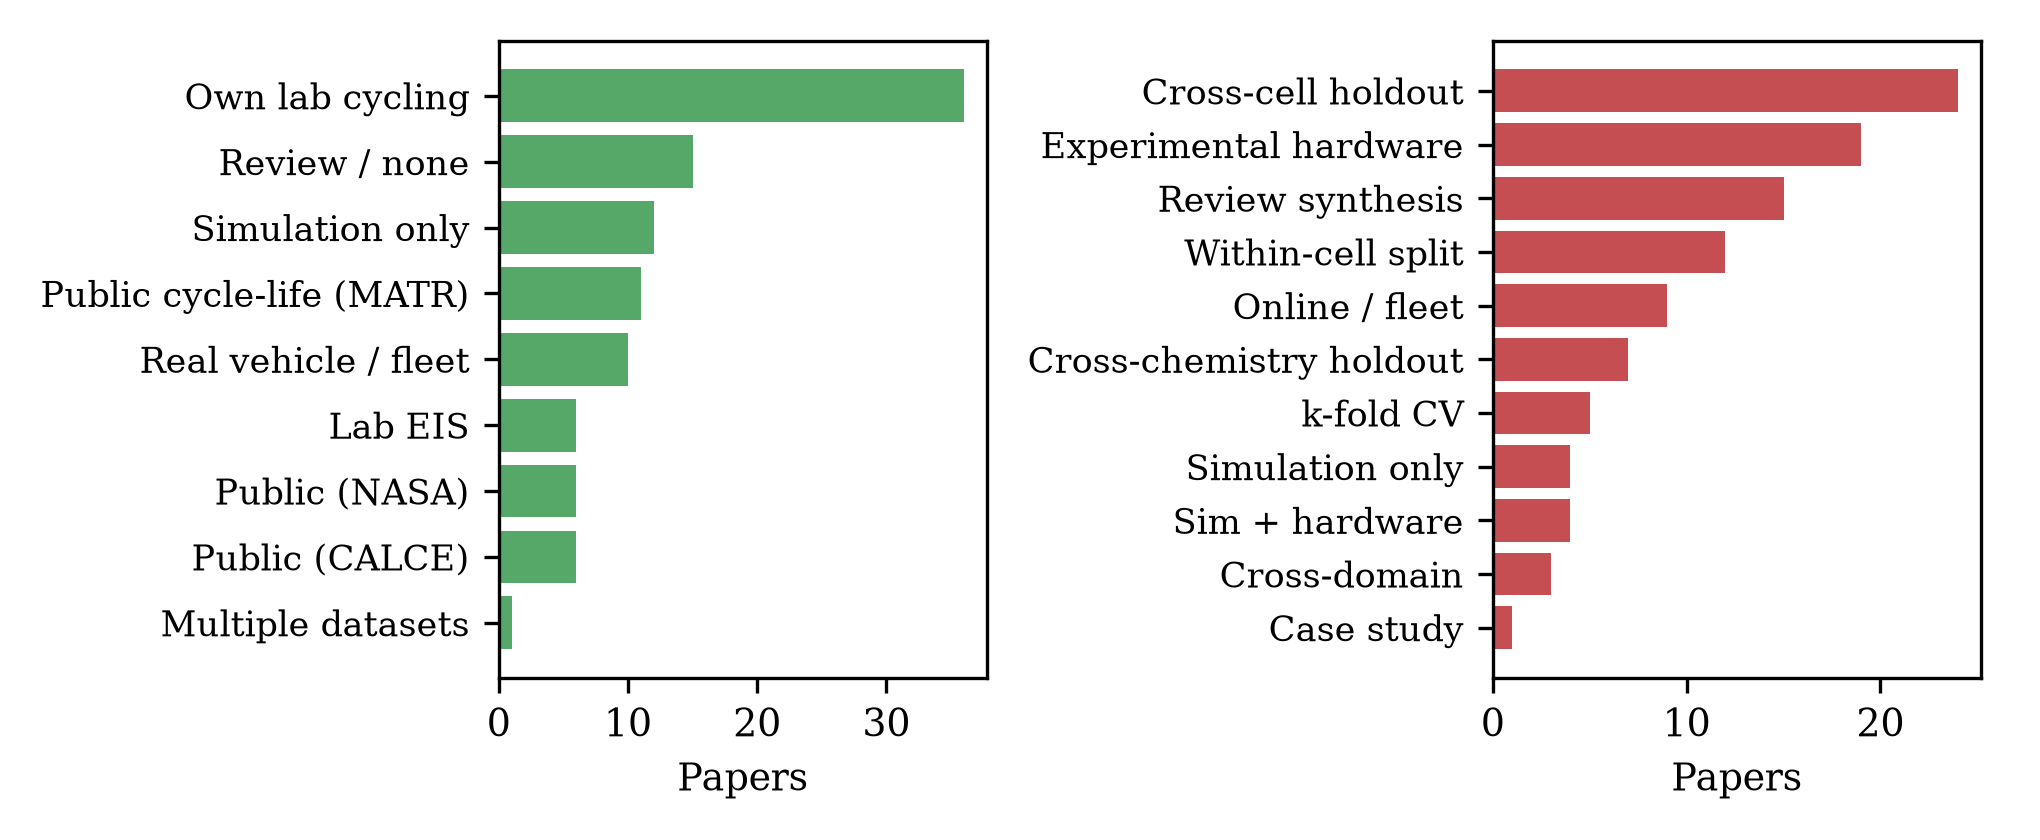
\includegraphics[width=6.8in]{figs/fig5_data_validation.png}
\label{fig:fig5_data_validation.png}
\end{figure*}

\begin{table*}[!t]
\caption{Benchmark datasets and data sources recurring across the corpus}
\label{tab:TABLE_DATASETS}
\centering
\footnotesize
\begin{tabular}{|p{2.35in}|p{0.40in}|p{3.89in}|}
\hline
\textbf{Data source} & \textbf{Papers} & \textbf{Typical use in corpus} \\
\hline
Own laboratory cycling & 36 & Primary training/testing data for estimators and protocols \\
Severson/Toyota--MIT--Stanford (MATR) & 11 & Cycle-life and early-life prediction benchmarks \\
NASA PCoE & 6 & Capacity-fade and RUL benchmarking \\
CALCE & 6 & SOH estimation and degradation modeling \\
Laboratory EIS & 6 & Impedance-based SOH/SOC and degradation-mode studies \\
Real vehicle / fleet data & 10 & Online SOH, anomaly detection, cloud BMS \\
Simulation (CFD/electrochemical) & 12 & Thermal design, charging optimization, runaway prediction \\
Review synthesis (no primary data) & 15 & Methodological and thematic reviews \\
Multiple datasets & 1 & Studies drawing on several of the above \\
\hline
\end{tabular}
\end{table*}

Validation practice deserves its own cross-tabulation because it moderates every accuracy claim in the corpus (Table 5). Cross-cell holdout --- training on some cells and testing on unseen siblings --- is the strongest widely used laboratory protocol (24 papers), and cross-chemistry or cross-domain transfer studies make the strictest demands (10 papers). At the weaker end, within-cell splits (12 papers) and unsupervised k-fold cross-validation (5 papers) leak trajectory information between train and test sets, producing optimistic errors that do not survive cell-to-cell variability; the review literature has long warned of this, and the corpus quantifies the warning. Experimental-hardware demonstrations (19 papers) and online or real-vehicle demonstrations (9 papers) anchor the strong end of the spectrum, and it is these --- not the largest architectures --- that carry the field's deployment evidence. Crossing validation practice with method family substantiates Section 3.2's remark with numbers: 13 of the 24 physics-informed/hybrid papers (54\%) use one of the strong protocols, against 49 of the other 67 primary-application papers (73\%) --- a physics prior does not, in itself, buy validation rigor.

\begin{table*}[!t]
\caption{Validation practices across the corpus}
\label{tab:TABLE_VALID}
\centering
\footnotesize
\begin{tabular}{|p{2.30in}|p{0.41in}|p{3.93in}|}
\hline
\textbf{Validation approach} & \textbf{Papers} & \textbf{Interpretation} \\
\hline
Cross-cell holdout & 24 & Strongest common laboratory protocol; unseen sibling cells \\
Experimental hardware & 19 & Physical validation of estimator or controller behavior \\
Review synthesis & 15 & No primary validation applicable \\
Within-cell split & 12 & Optimistic; trajectory leakage between train and test \\
Online / real-vehicle & 9 & Deployment-relevant evidence; rarest strong protocol \\
Cross-chemistry holdout & 7 & Strictest generalization demand in corpus \\
k-fold cross-validation & 5 & Optimistic without cell-level isolation \\
Simulation (+ hardware spot-check) & 8 & Model-fidelity dependent; strongest when hardware-checked \\
Cross-domain holdout & 3 & Transfer-specific evidence \\
Case study & 1 & Single-system demonstration \\
\hline
\end{tabular}
\end{table*}

\begin{table*}[!t]
\caption{Cross-tabulation of fleet-data use against online validation (103 papers). Fleet-data use describes the primary data source; online validation describes the validation protocol; their overlap is 8 of 10 fleet-data papers. The right-hand column pools the validation categories of Table 5.}
\label{tab:TABLE_FLEET}
\centering
\footnotesize
\begin{tabular}{|p{1.48in}|p{1.96in}|p{2.37in}|p{0.71in}|}
\hline
\textbf{} & \textbf{Online / real-vehicle validation} & \textbf{All other validation protocols (Table 5)} & \textbf{Total papers} \\
\hline
Real-vehicle / fleet data & 8 & 2 (transfer; case study) & 10 \\
Other data sources & 1 (laboratory-data demonstration) & 92 & 93 \\
Total & 9 & 94 & 103 \\
\hline
\hline
\end{tabular}
\end{table*}

Reading Fig. 6 and Tables 4 and 5 together yields the section's headline: the field's data supply is narrow, and its validation habits are calibrated to that narrowness. Public benchmarks made cumulative progress possible --- the Severson dataset alone catalyzed a family of early-prediction methods --- but they now also cap the credibility of reported generalization. The studies that escape this trap are precisely those that treat data sourcing and validation design as the research contribution: the multi-cell pipeline studies, the fleet-data health estimators, and the transfer-learning frameworks.

The concentration can be stated as a metric. Across 2019--2026, 23 corpus papers --- more than a fifth of the primary-application corpus --- rest on the same three public benchmarks (MATR, NASA, CALCE; Fig. 7). Because these benchmarks together contain on the order of a few hundred cells, the field's effective empirical sample has grown far more slowly than its publication count: output rose from single digits per year in 2019--2020 to 15--20 papers per year by 2023--2025, while benchmark-reuse kept pace step for step. We call this pattern benchmark saturation: the empirical base on which the community calibrates and compares estimators is approximately fixed while the literature multiplies on top of it, which inflates apparent comparability and hides dataset-specific failure modes.

\begin{figure*}[!t]
\caption{Benchmark saturation. Papers using the three dominant public benchmarks per year (stacked bars, left axis) against total corpus output per year (line, right axis). Benchmark reuse tracks publication growth throughout the window: the empirical base does not broaden as the literature multiplies.}
\centering

\includegraphics[width=5.1in]{figs/fig7_dataset_saturation.png}
\label{fig:fig7_dataset_saturation.png}
\end{figure*}

\subsection{Sensitivity analysis: does the journal-only corpus understate validation practice?}

Because the corpus excludes conference proceedings --- a major venue for control-oriented BMS work (CDC, ACC, IFAC, VPPC, ITEC) --- the validation findings of Section 3.4 could in principle be an artifact of venue selection: if conference papers systematically demonstrate more hardware and hardware-in-the-loop validation than journals, the journal-only sample would understate the field's actual practice. To test this, we curated a sensitivity set of 14 machine-learning battery papers from six control and transportation-electrification venues (ACC, ECC, CCDC, APEC, VPPC, ITEC, 2019--2025), retrieved by venue-scoped Crossref queries, restricted to proceedings articles, ranked by citation count, and verified by the same DOI-resolution procedure as the main corpus (released as conference\_sensitivity.csv). Validation practice was classified conservatively from the indexed abstracts by keyword screening into four classes: hardware/experimental stated, public dataset, simulation-level, and not stated.

\begin{table*}[!t]
\caption{Conference sensitivity set: 14 machine-learning battery papers from control and transportation-electrification venues (2019--2025), Crossref-verified, with validation evidence stated in their indexed abstracts.}
\label{tab:TABLE_CONF}
\centering
\footnotesize
\begin{tabular}{|p{0.53in}|p{0.48in}|p{3.50in}|p{2.01in}|}
\hline
\textbf{Venue (year)} & \textbf{Function} & \textbf{Method family (short)} & \textbf{Validation evidence stated in indexed abstract} \\
\hline
ITEC 2019 & SOC & LSTM recurrent network \cite{r28} & Not stated \\
VPPC 2021 & SOH & ML ensemble \cite{r29} & Public dataset \\
ITEC 2022 & SOC+SOH & Dual extended Kalman filter \cite{r30} & Not stated \\
ACC 2023 & SOC+SOH & Real-time estimator + batch least squares \cite{r31} & Not stated \\
ACC 2021 & SOC & Multiple-model adaptive estimation \cite{r32} & Simulation-level \\
ITEC 2023 & SOH & Histogram data + PCA + regression \cite{r33} & Public dataset \\
APEC 2023 & Overview & Review of ML-enabled estimation \cite{r34} & Not applicable \\
ECC 2021 & SOH & Reinforcement learning + observer \cite{r35} & Not stated \\
CCDC 2022 & SOH & CNN-BiLSTM transfer learning \cite{r36} & Hardware (stated); public data \\
VPPC 2019 & SOC & SVR + PCA with dual-polarization model \cite{r37} & Not stated \\
ACC 2024 & SOC+SOH & EKF critique and improvement \cite{r38} & Simulation-level \\
VPPC 2022 & Prognostics & ML on aging data \cite{r39} & Hardware (stated) \\
VPPC 2019 & SOC & Kalman filter on reduced electrochemical model \cite{r40} & Simulation-level \\
VPPC 2021 & SOC & Computationally efficient neural network \cite{r41} & Simulation-level \\
\hline
\end{tabular}
\end{table*}

The result supports representativeness rather than a venue gap. Only 2 of the 14 conference papers (14\%) state hardware or experimental validation in their indexed abstracts, 2 rest on public datasets, and 4 describe simulation-level validation --- against 19 of the 91 primary-application journal papers (21\%) with experimental-hardware demonstrations and a 68\% strong-protocol share (Table 5). Indexed abstract-level transparency about validation is, if anything, lower on the conference path, with 5 of 14 abstracts stating no validation basis at all. Two caveats bound this finding: conference abstracts are frequently truncated in bibliographic indexes, so the comparison measures stated evidence rather than underlying practice; and the sensitivity set is a curated sample, not a census. Within those bounds, however, the journal-only corpus does not understate the field's validation transparency --- and the observation that neither venue type reports validation systematically strengthens, rather than weakens, the case for the reporting standards proposed in Section 9.7.

\section{Machine Learning for Battery State Estimation}

\subsection{From filters to recurrent networks}

SOC estimation remains the most mature BMS function, and the corpus shows how machine learning entered it. The early-corpus pattern pairs learning with classical state estimation: Gaussian process regression for pack-level SOC with native uncertainty quantification \cite{r42}, and --- most influentially --- recurrent networks embedded in unscented Kalman filters, where the LSTM supplies a learned observation model and the filter supplies recursive correction \cite{r5}. Pure data-driven branches developed in parallel: support vector and ensemble regressors on engineered features benchmarked under automotive drive cycles \cite{r43}, and simulation-informed training pipelines that substitute automotive-accurate simulated data for exhaustive cell testing \cite{r44}. Reviews of this first generation conclude that deep-learning SOC estimation is accurate on well-sampled data but suffers from weak interpretability and inconsistent benchmarking \cite{r16}\cite{r17}.

A second generation tuned network structure itself. Particle-swarm-optimized LSTM improved accuracy and current-noise robustness over vanilla recurrent baselines \cite{r45}, and evolutionary-assisted CNN--BiLSTM hybrids report sub-1\% drive-cycle SOC errors \cite{r46}. This optimization-augmented family illustrates a recurring pattern of the corpus: gains are real but modest, and the meta-heuristic component is tuned offline while adding training cost --- an investment that only pays at deployment if the estimator's life is long. Robustness-oriented work addresses pack heterogeneity directly, jointly estimating pack SOC and cell inconsistency with balancing-aware formulations \cite{r47}, large-format applications extend estimation to containerized energy-storage strings with relaxed sensing \cite{r48}, unified frameworks estimate SOH and SOC jointly from partial charging data \cite{r49}, and comparative benchmarks weigh accuracy against the computational budget of electrified powertrains \cite{r50}\cite{r51}.

Two features of this cluster stand out against the rest of the corpus. First, it is the only function where classical estimation theory and machine learning have genuinely fused in published practice: the filter-embedded pattern \cite{r5} recurs across the five-year window in increasingly sophisticated forms, whereas health estimation and prognostics largely abandoned hybrid filtering after their Gaussian-process phase. Second, SOC papers report the corpus's most standardized evaluation --- drive-cycle profiles at room temperature with RMSE or MAE in percent SOC --- which makes their benchmarks legible even where the underlying datasets remain private. The cost of that legibility is convergence: with every paper evaluating on the same standard cycles, the marginal contribution of a new architecture is shrinking, and the cluster's research attention is shifting toward robustness conditions --- noise, sensor faults, temperature, and aging shift --- where the standard benchmarks are silent.

\subsection{Hybrid and physics-informed estimation}

The most substantive recent shift in SOC estimation is the move from purely learned estimators to hybrid schemes in which a filter, an equivalent-circuit model, or a physics prior constrains the learner. GA-optimized LSTM networks coupled with improved adaptive Kalman filtering reach low error under measurement noise that breaks pure-network estimators \cite{r52}; equivalent-circuit-informed ML on impedance features estimates SOC across temperatures \cite{r53}; and physics-informed recurrent structures embed battery dynamics directly into the network's training objective \cite{r10}. These schemes trade engineering complexity for extrapolation behavior: because the physics component carries structure that does not need to be relearned, hybrid estimators degrade more gracefully outside their training envelope --- the property that matters most onboard.

\subsection{Critical assessment}

The SOC literature of the corpus is accurate but inward-looking. Reported errors are now consistently below 1--2\% SOC on the standard drive cycles, yet 13 of the 17 corpus SOC papers rest on laboratory-scale data and 12 on a single chemistry under curated profiles, and only one demonstrates fleet-scale operation \cite{r48}. The review literature itself identifies the consequence: benchmark heterogeneity makes cross-paper comparison nearly meaningless, and generalization across temperature, chemistry, and aging state remains weakly evidenced \cite{r20}. The SOC function is, in other words, an area where the research problem has largely been solved on laboratory terms but the deployment problem --- guaranteed accuracy on arbitrary packs over full aging --- has not.

State estimation is also where the corpus's two sensing-hardware threads meet the software thread. Impedance-based SOC estimation demonstrates that electrochemical information beyond terminal voltage can drive estimation when EIS is available \cite{r53}, while the ultrasonic-sensing line proposes non-electrical channels that could in principle be integrated into pack hardware at automotive cost \cite{r54}. Both remain laboratory-bound for cost and durability reasons, but they mark the boundaries of a design space --- better software on existing sensors versus new sensors for better software --- that the wider BMS industry is actively exploring.

\section{Machine Learning for Health Estimation and Prognostics}

\subsection{Feature engineering and classical estimators}

SOH estimation and RUL prediction form the largest functional block of the corpus (35 papers). The founding pattern is classical: extract health-sensitive features from partial charge or discharge curves, then regress with Gaussian process or similar shallow models. Incremental-capacity analysis with Gaussian process regression established the template with explicit uncertainty bounds \cite{r55}; differential thermal voltammetry extended the feature space to thermal signatures \cite{r56}; and deep Gaussian processes coupled capacity prognosis with degradation-mode identification \cite{r57}. Relaxations of the measurement burden followed: random partial charging data proved sufficient for accurate SOH \cite{r58}, and charging-segment adjustment refined features for vehicle-level use \cite{r59}. The landmark systematization of this generation is the 179-cell machine-learning pipeline of Roman et al., which showed that relaxed charge-curve features support accurate, uncertainty-quantified SOH estimation across a heterogeneous commercial-cell fleet \cite{r60}.

The feature taxonomy underlying this generation is worth making explicit because it explains both the cluster's strengths and its brittleness. Incremental capacity and differential voltage features transform charge curves into peaks whose positions and areas track degradation mechanisms; differential thermal voltammetry adds the temperature dimension; and partial-charging features deliberately sacrifice completeness for practicality, accepting any sufficiently informative voltage window. The approach assumes that the feature-to-health mapping is stable across the cells used for training --- an assumption that holds within a cell model and laboratory but weakens across manufacturers, formats, and field profiles. The 179-cell pipeline study is important precisely because it tested that assumption at fleet scale within one commercial technology, and its success should not be over-read as license to transfer features across technologies \cite{r60}.

\subsection{Deep sequence and cross-cell models}

Deep architectures entered prognostics as sequence models over capacity-fade trajectories and as representation learners over raw curves. Graph convolutional networks fuse multiple health indicators for joint SOH/RUL prediction \cite{r7}; BiLSTM--Transformer hybrids track health under the specific stress of fast charging \cite{r8}; hybrid-fusion networks target real-time prediction streams \cite{r61}; graph neural networks over partial discharge curves improve cross-cell generalization \cite{r62}, and interpretable deep learning couples accuracy with transparency mechanisms \cite{r63}. A particularly important line uses real-world vehicle data rather than laboratory cycling, demonstrating that deep estimators can absorb field-data noise \cite{r6}, and pack-level fusion methods now estimate SOH directly from fleet charge streams \cite{r64}. At the field's high end, a Nature Communications study showed that deep models can estimate SOH without additional degradation experiments by learning trajectory features that generalize across chemistries \cite{r65}.

\subsection{Early-life prediction}

Early-life prediction --- forecasting lifetime from the first cycles --- is the corpus's most consequential methodological export to practice, because it compresses test times from months to days. Beyond the founding study \cite{r3}, charge-process features predict cycle life across diverse duty cycles \cite{r66}, ML frameworks extract lifetime information from formation-style tests \cite{r67}, hybrid physics-plus-learned models give early RUL from limited cycles \cite{r68}, and discharge-voltage features extend the approach to lithium-metal chemistries \cite{r69}. Board-level implementations close the loop to hardware, predicting capacity and RUL on embedded platforms in real time \cite{r70}.

The economics of early-life prediction explain its rapid uptake: formation and initial cycling are already performed on every production cell, so early-prediction features are available for free at the point of manufacture, and warranty structuring, second-life triage, and cell matching all become data products. The methodological caveat is selection: cells that reach the secondary market, and cell batches that survive manufacturing screens, are conditioned samples whose early-cycle feature distributions differ from the training population. No corpus paper yet quantifies this survivorship effect, which makes it one of the more consequential open measurement problems in the cluster.

\subsection{Physics-informed and hybrid prognostics}

The prognostics cluster shows the corpus's most visible physics-informed turn. Physics-informed online degradation models support proactive health management by embedding degradation structure into learned models \cite{r71}; physics-informed hybrid reinforcement learning reduces the data demand of SOH estimation \cite{r72}; a generalizable PINN achieves cross-cell SOH estimation from limited early-cycle data \cite{r73}; EIS-informed physics-constrained networks estimate SOH from small impedance datasets \cite{r74}; and a generic physics-informed framework predicts RUL from small early-life samples across datasets \cite{r75}. Multi-feature hybrid schemes lift RUL accuracy across datasets \cite{r76}, signal-decomposition hybrids sharpen capacity-fade prediction on noisy series \cite{r77}, and deep reinforcement learning adaptively selects prognostic models along aging trajectories \cite{r13}. The shared motivation is clear: pure data-driven models extrapolate poorly past their training envelope, and physics priors are the cheapest available source of structure.

\subsection{Transfer learning and cross-domain generalization}

Transfer learning addresses the corpus's central weakness --- generalization --- directly. Domain-adversarial training adapts SOH estimators across operating conditions without target-domain labels \cite{r11}; deep transfer learning with partial charging curves carries capacity estimation across cell types \cite{r12}; transfer under fast-charging protocols extends the approach to protocol shift \cite{r78}; transfer-learning-based EIS estimation crosses chemistries \cite{r79}; and a general framework quantifies and manages the laboratory-to-fleet domain gap for trained estimators \cite{r80}. Framework-level work consolidates these threads: real-time online feature extraction from vehicle data \cite{r81} and reviews charting non-probabilistic estimation techniques \cite{r18}, alongside joint SOH/RUL architectures that fuse multiple health indicators \cite{r7}.

\subsection{Critical assessment}

Prognostics is where the corpus's validation problem bites hardest. Accuracy claims cluster around SOH errors of 1--2\% and RUL errors of tens of cycles, but these are established overwhelmingly on public benchmark cells: the Severson-MATR dataset alone appears in 11 corpus papers, NASA and CALCE in 12 more. Within-cell splits and k-fold protocols --- which leak trajectory information between train and test --- account for 10 of the 35 primary studies in the health-prognostics complex, and for 17 of the corpus as a whole. The transfer-learning papers are the honest exception, in that their whole object is distribution shift; but they also reveal how much shift remains unaddressed, with negative transfer cases and per-protocol fine-tuning acknowledged but rarely resolved. The mature judgment is that SOH estimation under controlled conditions is approaching incremental returns, while the prognostics problem that matters --- calibrated lifetime and safety margins for arbitrary packs in the field --- remains open \cite{r2}\cite{r19}.

Metric heterogeneity compounds the validation problem. SOH papers report RMSE or MAE in percent capacity, sometimes normalized differently; RUL papers report cycle counts, percentages of true life, or knee-point errors defined against arbitrary end-of-life thresholds; charging papers report charge time, energy efficiency, and capacity retention after fixed cycle counts, which conflate estimation error with protocol quality. No two clusters share a metric, and within clusters the definitions vary enough that a quantitative meta-analysis of pooled accuracy --- the trademark move of clinical meta-research --- is not defensible for this literature. The qualitative synthesis of Sections 4--8 is therefore organized around method families, data regimes, and validation designs rather than around pooled effect sizes; this is a deliberate methodological choice, and readers should treat any cross-paper accuracy table with corresponding caution.

\section{Machine Learning for Charging Control and Optimization}

\subsection{Closed-loop optimization of charging protocols}

Charging control is the function where machine learning has changed experimental practice most directly, not merely what can be estimated. The defining result is Attia et al.: a Bayesian optimization loop over charging-protocol parameters, evaluating candidate protocols through continuous cycling, identified protocols charging cells to 80\% in around 10 minutes within 2.5 months --- against roughly 18 months for the equivalent manual search \cite{r4}. The significance is methodological as much as practical: closed-loop learning converts protocol design from expert iteration into sample-efficient optimization. Subsequent work broadened the objective space. Ensemble surrogate models make model-based charging-strategy optimization tractable under multi-objective trade-offs \cite{r82}, and data-driven Bayesian fast-charging optimization reduces charge time under explicit degradation constraints \cite{r83}.

\subsection{Learning to charge around degradation physics}

A second line embeds degradation mechanisms into the charging decision itself. Machine-learning fast charging that perceives and regulates internal lithium-plating onset enables plating-free rapid protocols that violate conventional voltage-safe schedules with impunity \cite{r84}. Adaptive multistage constant-current schemes adjust stage boundaries online against measured degradation \cite{r85}, and module-level optimization manages temperature gradients across packs during charging \cite{r86}. Pack-level extensions coordinate balance-aware charging for imbalanced strings \cite{r87} and multi-objective meta-heuristic schemes negotiate charge time against temperature rise and aging \cite{r88}.

Scale effects are the cluster's frontier. Cell-level protocols do not compose into pack-level schedules, because cell-to-cell variability makes the weakest cell the binding constraint; module-level optimization with temperature-gradient constraints \cite{r86} and balance-aware pack charging \cite{r87} are the corpus's first responses. The control-theoretic gap is equally important: optimization produces open-loop schedules, while deployment wants closed-loop policies that react to measured state --- which is precisely where the reinforcement-learning line, still under-represented in journal-grade hardware validation, is expected to grow.

\subsection{Critical assessment}

Charging is also where the gap between demonstration and deployment is most concrete. The corpus contains eight charging papers; of these, one is a large-scale closed-loop hardware campaign \cite{r4}, three validate on laboratory hardware, and the remainder are simulation-only or optimization-method demonstrations. RL-based charging strategies --- a substantial adjacent literature --- are underrepresented here precisely because most are validated in simulation against electrochemical models. The unsolved problem is certifiable learning-based charging: a controller that adapts to cell-to-cell variability and aging in production vehicles must carry a safety argument that current model-free learners cannot yet make, which is why mechanism-aware schemes such as plating-perception control \cite{r84} are the most deployment-relevant results in this cluster.

\begin{table*}[!t]
\caption{Representative corpus studies by management function and method family. Entries gloss each study as: study summary (data basis; headline contribution). References in brackets refer to the numbered list.}
\label{tab:TABLE3}
\centering
\footnotesize
\begin{tabular}{|p{1.01in}|p{2.11in}|p{3.52in}|}
\hline
\textbf{Function} & \textbf{Method family} & \textbf{Representative studies (data; contribution)} \\
\hline
State estimation (SOC) & Filter-embedded learning; meta-heuristic DL & LSTM+UKF embedded estimator (laboratory cells; learned observation model in a UKF) \cite{r5}; PSO-LSTM (laboratory cells; meta-heuristically tuned recurrent SOC) \cite{r45}; GA-LSTM with adaptive Kalman filtering (laboratory cells; low error under noise) \cite{r52} \\
Health estimation (SOH) & Classical ML; deep learning; transfer learning & ML pipeline over 179 cells (own cell fleet; relaxed charge-curve features) \cite{r60}; deep learning without extra degradation experiments (public MATR dataset; cross-chemistry generalization) \cite{r65}; real-world vehicle SOH (fleet data; field-noise robustness) \cite{r6} \\
Prognostics (RUL) & Classical ML; physics-informed; RL & Early-life cycle prediction (public MATR dataset; about 9\% median test error) \cite{r3}; physics-informed early-cycle RUL (multiple datasets; small-data prognosis) \cite{r75}; deep-RL prognostic model fusion (public NASA dataset; adaptive model selection) \cite{r13} \\
Charging control & Bayesian optimization; mechanism-aware control & Closed-loop Bayesian protocol optimization (hardware prototype; 2.5 versus 18 months to a protocol) \cite{r4}; plating-perceiving fast charging (hardware prototype; plating-free protocols) \cite{r84}; ensemble-surrogate charging optimization (laboratory cells; multi-objective strategies) \cite{r82} \\
Thermal management & ANN surrogate; physics-informed; optimization & ANN temperature prediction (laboratory cells; low-error thermal model) \cite{r89}; PINN heat-generation estimation (simulation; embedded thermal physics) \cite{r9}; ML-assisted BTMS design (simulation; multi-objective cooling design) \cite{r90} \\
Fault \& safety & Shallow ML; multiphysics + ML; transfer learning & SVM fault diagnosis (hardware prototype; sensor and connection faults) \cite{r91}; multiphysics-ML runaway prediction (simulation and hardware; module-level hazard) \cite{r92}; cross-fleet runaway-diagnosis transfer (fleet data; small-sample diagnosis) \cite{r93} \\
Cross-cutting & Physics-informed; XAI; digital twin; LLM & EIS diagnostics PINN review (multiple studies; paradigm synthesis) \cite{r21}; uncertainty-aware early-life prediction (public MATR dataset; calibrated forecasts) \cite{r94}; LLM vehicle-cloud management (fleet data; orchestration layer) \cite{r15} \\
\hline
\end{tabular}
\end{table*}

\section{Machine Learning for Thermal Management, Faults and Safety}

\subsection{Thermal-state estimation and thermal management}

Thermal management is the corpus's smallest quantitative engineering cluster (8 papers) but a disproportionately safety-critical one. Data-driven temperature estimation ranges from ANN models predicting cell temperature across operating conditions \cite{r89} to internal-temperature sensing under ultrahigh-rate discharge, where surface measurement fails \cite{r95}. On the design and control side, ML-surrogate models accelerate liquid-cooling plate analysis and multi-objective optimization of BTMS geometry \cite{r96}\cite{r90}, experimentally validated parallel-liquid-cooling designs demonstrate the optimization loop end-to-end \cite{r97}, and ANN-controlled thermal management reduces cooling parasitic load while holding temperature limits \cite{r98}. Physics-informed heat-generation estimation embeds thermal physics priors into the learning problem \cite{r9}, and a state-of-the-art review consolidates the cluster \cite{r25}.

The thermal cluster's papers divide cleanly by purpose, and the division clarifies where machine learning adds value. For \textit{estimation} purposes --- predicting internal or surface temperature under load --- learned models replace thermocouple instrumentation that no production pack can afford, and physics-informed variants regularize the extrapolation regime where data-driven thermal models are least trustworthy \cite{r9}. For \textit{design} purposes --- sizing and arranging cooling hardware --- ML surrogates amortize expensive CFD evaluation across optimization loops, turning weeks of simulation into tractable search \cite{r96}\cite{r90}. For \textit{control} purposes --- modulating cooling effort online --- ANN controllers demonstrate parasitic-load reductions in simulation \cite{r98}, but no corpus paper yet closes this loop on hardware, leaving thermal control where charging control was five years ago.

\subsection{Fault diagnosis and anomaly detection}

Fault and safety applications (9 papers) divide into diagnosis of realized faults and prediction of impending hazards. On the diagnosis side, grid-search-optimized support vector machines classify sensor and connection faults \cite{r91}, curvilinear-Manhattan-distance methods detect multiple pack fault types in operating fleets \cite{r99}, and multi-scenario deep anomaly detection covers real EV operating envelopes \cite{r100}. Manufacturing-side inspection applies force-signal deep learning to catch lithium-plating-type defects before cells ship \cite{r101}. The hazard-prediction side is increasingly model-based: multiphysics models coupled with ML predict module-level thermal-runaway progression \cite{r92}, a multiphysics-informed DeepONet predicts runaway using virtual data to augment scarce experimental events \cite{r102}, and multi-source domain transfer moves thermal-runaway diagnosis across vehicle fleets with small target samples \cite{r93}.

\subsection{Critical assessment}

Safety applications carry the corpus's highest stakes and its thinnest evidence base. Thermal-runaway events are rare and expensive to generate, so learning systems train on simulation or small laboratory campaigns; the DeepONet line's virtual-data approach \cite{r102} is a rational response, but it inherits the fidelity limits of the underlying multiphysics models. The reviews in this cluster are notably candid: laboratory fault diagnosis has historically failed to transfer to real vehicles because fault signatures are masked by pack-level averaging, sensor noise, and operating diversity \cite{r24}\cite{r23}. The fleet-data anomaly-detection studies are therefore the cluster's most valuable trend, even though label scarcity for rare faults keeps evaluation largely qualitative.

\section{Cross-Cutting Directions}

\subsection{Physics-informed learning}

Physics-informed and hybrid model--data learning is the corpus's largest and fastest-rising methodological theme (24 papers across all functions). Beyond the prognostics applications of Section 5.4, physics-informed structures appear in state estimation \cite{r10}\cite{r103}, heat-generation estimation \cite{r9}, and impedance-based diagnostics, where physics-informed deep learning over electrochemical impedance spectra is consolidating into a diagnostic paradigm of its own \cite{r21}. Physics-constrained autoencoders improve health prediction over purely learned counterparts \cite{r104}, and recurrent networks trained to anticipate uncertain future duty conditions address degradation prediction under distribution shift directly \cite{r105}. A parallel fusion literature combines physical and data-driven models for internal-state estimation generally \cite{r106}. The appeal is easy to state: physics priors supply exactly the extrapolation structure that pure learners lack. The corpus's caution is that most physics-informed studies embed \textit{simplified} physics --- equivalent-circuit or reduced electrochemical models --- so the hybrid inherits model bias even as it gains structure.

\subsection{Interpretability and uncertainty}

A smaller but consequential cluster makes learning systems inspectable. Explainability-driven feature selection improves SOH estimator robustness via SHAP analysis \cite{r107}; interpretable ML links manufacturing coating parameters to cell capacity, connecting management analytics to production \cite{r108}; interpretable hybrid ML untangles co-evolving degradation chemistries in lithium--sulfur cells \cite{r109}; and uncertainty-aware, explainable models deliver calibrated early-life predictions \cite{r94}. Review-level retrospectives of interpretable battery prognosis now chart the theme's trajectory \cite{r22}. The state of practice remains, however, dominated by post-hoc explanation of otherwise black-box models --- a necessary but not sufficient condition for the safety certification that onboard ML will eventually require.

The uncertainty thread deserves separate emphasis because it is the certification-relevant one. Gaussian-process lineages carry calibrated intervals as a first-class output \cite{r55}, the uncertainty-aware early-prediction study demonstrates calibrated lifetime distributions rather than point forecasts \cite{r94}, and conformal-style guarantees are beginning to appear in adjacent prognostics work. The interpretability thread, by contrast, remains dominated by post-hoc attribution (SHAP-style) analyses that explain \textit{which features mattered} without bounding \textit{what the model will do} on out-of-distribution inputs. For safety cases the two are not substitutes: attribution supports debugging and trust-building, while calibrated uncertainty supports decision rules --- and only the latter has a route into certification argument.

\subsection{Digital twins, cloud BMS, and new sensing}

System-level architecture is emerging as a research object in its own right. Digital-twin implementations track individual battery aging through incremental learning \cite{r110} and couple LSTM surrogates with real-time thermal observation \cite{r111}; cloud-based platforms perform in-situ life prediction and classification at fleet scale from streaming charge data \cite{r112}; and second-life workflows use impedance-based accelerated SOH estimation to triage retired packs \cite{r113}. Non-electrical sensing broadens the measurement base: ultrasonic signatures processed with ML provide a SOC channel orthogonal to voltage sensing \cite{r54}, impedance-spectroscopy ML supports SOC and SOH estimation despite EIS's onboard-cost problem \cite{r53}\cite{r114}, and battery state-of-power estimation combines learned models with numerical search for real-time capability prediction \cite{r115}.

The twin/cloud/second-life cluster carries the corpus's most concrete systems implications. Digital-twin formulations reframe estimation as continual model maintenance --- the incremental-learning requirement follows from pack heterogeneity and aging drift \cite{r110} --- and cloud architectures relocate heavy computation off-vehicle, at the price of connectivity dependence and data-volume engineering \cite{r112}. Second-life workflows invert the deployment direction: instead of bringing estimators to new cells, they bring cheap, accelerated assessment to aged, heterogeneous cells \cite{r113}, where classification-style decisions (deploy, repurpose, recycle) tolerate coarser resolution than onboard safety estimation. These three settings differ in latency budgets, error tolerance, and update cadence --- and the corpus suggests the field is beginning to design for those differences rather than for a single notion of ``the BMS.''

\subsection{Foundation models and LLM-based management}

The corpus's youngest theme is generative: domain-specific large language models perform risk analysis of battery energy-storage incidents by synthesizing heterogeneous incident reports \cite{r14}, and domain-knowledge-enhanced LLM agents orchestrate vehicle-cloud collaborative battery management \cite{r15}. These first studies position LLMs as reasoning and coordination layers above numerical estimators rather than as estimators themselves --- a sensible division given that hallucination risk is intolerable in safety-critical state estimation. Their appearance in mainstream energy journals in 2025--2026 nonetheless marks a new phase: the management stack is beginning to absorb foundation-model components, and the corpus's method-evolution data (Fig. 4) suggest the field expects this line to grow.

Because BMS software is safety-critical, this review positions foundation models not as better estimators but as orchestration layers, and it is worth making the division of labor explicit. Table 9 contrasts established practice for classical and deep learning estimators with what the first LLM studies actually demonstrate, and states the guardrails this review regards as mandatory before any LLM component touches a safety-relevant path. The right-hand column is normative guidance proposed here, not claims about the published studies; the published LLM work to date is confined to risk analysis and coordination, which is exactly where it belongs at this stage.

\begin{table*}[!t]
\caption{Safety and verification taxonomy for foundation-model components in the BMS stack. The right-hand column is normative guidance proposed by this review, not claims about the published studies.}
\label{tab:TABLE_LLM}
\centering
\footnotesize
\begin{tabular}{|p{0.57in}|p{1.64in}|p{2.16in}|p{2.16in}|}
\hline
\textbf{Dimension} & \textbf{Classical / deep ML estimators (established practice)} & \textbf{Published LLM studies (2025--2026)} & \textbf{Required guardrail (this review)} \\
\hline
Role in the stack & Calibrated numeric estimation and detection & Incident risk analysis \cite{r14}; vehicle-cloud orchestration \cite{r15} & Estimation stays with calibrated ML; LLM coordinates, summarizes, explains \\
Grounding & Trained on domain cycling data & Domain-tuned corpora and knowledge-enhanced prompting & Retrieval over verified corpora with source citations; no ungrounded recall \\
Dominant failure mode & Bounded numeric error under distribution shift & Open-ended hallucinated text & Outputs restricted to structured, checkable forms; never free text into protection logic \\
Uncertainty & Gaussian-process / conformal intervals in a subset of studies & Not quantified in published studies & Calibrated intervals mandatory before any actuation-adjacent role \\
Latency and compute & Millisecond-class, onboard & Second-class, cloud-dependent & Offline analysis and planning only unless real-time evidence is shown \\
Safety authority & Bounded by physics envelopes and thresholds & Undefined in published studies & LLM components must never hold direct cell-level protection authority \\
\hline
\end{tabular}
\end{table*}

\subsection{Manufacturing analytics and system-level synthesis}

Two further cross-cutting threads connect management to the wider battery value chain. Cell-production mapping studies chart ML use across manufacturing stages from mixing to formation \cite{r116}, complementing the coating-quality interpretability work \cite{r108} and manufacturing defect detection \cite{r101} --- the management implication being that cell quality information is itself a BMS input. And the pack-level insight that routine cell balancing can be eliminated in well-managed packs, reducing hazardous lithium-plating side reactions, shows learned analysis reshaping a function (balancing) that classical control had considered settled \cite{r27}, while ML mappings from equivalent-circuit parameters to electrochemical properties give classical BMS models a physically interpretable learned layer \cite{r117}.

\section{Research Gaps and Future Directions}

Cross-referencing the bibliometric analysis of Section 3 with the function-level reviews of Sections 4--8 yields six structural gaps, discussed in Sections 9.1--9.6, summarized in Table 10, and then operationalized into a concrete reporting checklist in Section 9.7.

\subsection{Validation and benchmarking standards}

The corpus's validation data are unambiguous: 17 primary studies corpus-wide use within-cell splits or unsupervised k-folds, and only 9 of all 103 papers demonstrate their systems online or on real fleets. Until cross-cell, cross-temperature, and cross-protocol holdout protocols become reporting norms, published accuracy figures will keep overstating deployable performance. The most valuable near-term contribution the community can make is standardized transfer protocols --- train-on-chemistry-A/test-on-chemistry-B, train-on-lab/test-on-fleet --- reported alongside headline accuracy, as already practiced by the transfer-learning and general-framework studies \cite{r80}\cite{r79}.

A second standardization target is reporting itself. The corpus's papers rarely disclose split definitions, random seeds, or compute budgets --- omissions that make independent replication laborious and meta-analysis impossible (Section 5.6). A community-endorsed reporting checklist --- dataset identity and version, split protocol, uncertainty quantification, and hardware context --- would cost little and would let the synthesis literature do its job.

\subsection{Data sharing and the benchmark monoculture}

Eleven corpus papers rest on a single public dataset (Severson-MATR), and NASA and CALCE sustain much of the remainder; 35 papers use private laboratory cells whose data are not released. The monoculture inflates apparent comparability and hides dataset-specific failure modes. Federated learning over fleet data, standardized anonymized fleet-data releases, and multi-institution cycling campaigns --- in the spirit of the 179-cell pipeline \cite{r60} --- would diversify the evidence base at modest incremental cost.

The economics argument strengthens the technical one. A fleet operator's marginal value from a percentage point of SOH accuracy is measured in warranty provisions and residual-value pricing, which justifies onboard compute budgets that academic prototypes routinely ignore. Quantized and pruned recurrent models, event-driven inference triggered by charge sessions rather than continuous streams, and asymmetric architectures --- lightweight onboard estimators with cloud-side retraining --- are the concrete design patterns emerging from the corpus's edge-aware minority \cite{r70}\cite{r81}.

\subsection{Edge deployment and onboard constraints}

Only a handful of corpus works treat onboard compute, memory, or latency as first-class design constraints, notably the board-level RUL implementation \cite{r70} and real-time feature-extraction studies \cite{r81}. The gap is widening as models grow: transformer and PINN architectures trained on workstations must eventually run beside BMS microcontrollers. Quantization-aware training, neural architecture search under resource constraints, and hybrid designs that place heavy learners in the cloud and lightweight correction layers onboard are the natural research program here \cite{r15}.

\subsection{Trust: uncertainty, interpretability, and certification}

Estimates that guide protection and charging decisions need calibrated uncertainty and auditable reasoning. The corpus's uncertainty-aware \cite{r94}, explainability-driven \cite{r107}, and Gaussian-process lineages \cite{r55} point the way, but certification-grade ML --- models whose failure modes are enumerated and bounded --- remains beyond the published state of the art. Hybrid physics--data architectures are the most credible certification path because part of their behavior is analytically specified; making that argument rigorous is an open task for the PINN community.

\subsection{Foundation-model integration}

The first LLM-based management studies \cite{r14}\cite{r15} suggest a division of labor worth formalizing: foundation models as reasoning, orchestration, and human-interface layers; conventional ML as calibrated estimators; physics models as safety envelopes. Research is needed on grounding (preventing hallucinated battery knowledge), latency, and the division of safety authority between learned and non-learned components. Battery-domain foundation models pretrained on cycling corpora are a plausible medium-term development.

\subsection{Under-served functions}

Finally, the function distribution itself signals opportunity. Cell balancing is nearly untouched by ML beyond pack-level insight \cite{r27}; charging control needs certifiable adaptive protocols; and thermal management remains simulation-dominated \cite{r25}. These functions share a property that explains their under-representation: they are \textit{control} problems, where errors act on the battery rather than merely reporting on it, and where the evidence bar is correspondingly higher. Closing them will require the safety-case machinery of Section 9.4 as much as new algorithms.

\begin{table*}[!t]
\caption{Structural research gaps and corresponding future directions}
\label{tab:TABLE_GAPS}
\centering
\footnotesize
\begin{tabular}{|p{0.99in}|p{2.83in}|p{2.83in}|}
\hline
\textbf{Gap} & \textbf{Evidence in corpus} & \textbf{Future direction} \\
\hline
Validation practice & 17 primary studies use within-cell or k-fold validation; 9/103 demonstrate online or fleet use & Standardized cross-cell, cross-chemistry, lab-to-fleet transfer protocols as reporting norms \\
Benchmark monoculture & Single public dataset underlies 11 studies; NASA/CALCE sustain much of the rest & Federated learning, anonymized fleet-data releases, multi-institution cycling campaigns \\
Onboard deployment & Few studies treat compute/memory/latency as design constraints & Quantization-aware training, resource-constrained NAS, cloud--edge hybrid estimation \\
Trust and certification & Interpretability mostly post-hoc; uncertainty rarely calibrated & Calibrated uncertainty, analytically specified hybrid architectures, safety-case methodology \\
Foundation-model integration & First two LLM-based studies appear 2025--2026 & Grounded LLM orchestration layers; domain foundation models; division of safety authority \\
Under-served functions & Balancing (2 papers), charging control (8), thermal (8) & Certifiable adaptive control with mechanism-aware safety envelopes \\
\hline
\end{tabular}
\end{table*}

\subsection{A reporting checklist for machine-learning BMS studies}

The most concrete artifact this review can offer is procedural. Modeled on the CONSORT and PRISMA checklists that transformed reporting in clinical and review literature, Table 11 proposes a twelve-item BMS-ML reporting checklist: the minimum metadata a study should disclose for its accuracy claims to be comparable, reproducible, and poolable in future syntheses. None of the items is onerous; each corresponds to a practice whose absence the corpus analysis showed to be distorting --- undisclosed splits (Section 3.4), uncalibrated uncertainty (Section 8.2), unnamed datasets (Section 3.4), or unquantified compute (Section 9.3). We suggest journals adopt it as a submission checklist and that authors attach it to their released datasets.

\begin{table*}[!t]
\caption{Proposed BMS-ML reporting checklist (BMS-ML-RC), modeled on CONSORT/PRISMA reporting standards.}
\label{tab:TABLE_CHECKLIST}
\centering
\footnotesize
\begin{tabular}{|p{0.37in}|p{1.71in}|p{4.56in}|}
\hline
\textbf{\#} & \textbf{Reporting item} & \textbf{What must be reported} \\
\hline
1 & Dataset identity & Exact name and version of every dataset (e.g., Severson-MATR, NASA, CALCE); download source \\
2 & Cell population & Number of cells, chemistry, manufacturer, format, and batch for every training and test set \\
3 & Sensor and sampling context & Measured channels, sampling rate, sensor class, and temperature conditions \\
4 & Split protocol & Split type (within-cell / cross-cell / cross-chemistry / cross-domain) and isolation argument; within-cell splits must be flagged as such \\
5 & Out-of-distribution evaluation & At least one protocol under which test conditions differ from training (chemistry, temperature, protocol, or source) \\
6 & Baselines & At least one classical baseline alongside the proposed architecture, with identical data \\
7 & Randomness control & Seeds or repeated-run statistics for every stochastic training result \\
8 & Uncertainty & Calibrated uncertainty or error bars for headline claims, not point estimates alone \\
9 & Compute budget & Training compute and inference latency/memory on the target (or a stated reference) platform \\
10 & Failure analysis & At least one documented failure mode and its distribution (where the model is worst) \\
11 & Validation environment & Which of the following applies: simulation, laboratory cycling, hardware prototype, online/fleet \\
12 & Artifact availability & Data and code deposit (DOI-backed) or an explicit stated exemption \\
\hline
\end{tabular}
\end{table*}

\begin{figure*}[!t]
\caption{Milestones of machine learning in battery management, 2019--2026, drawn from the corpus: early-life cycle prediction \cite{r3}, closed-loop Bayesian fast charging \cite{r4}, fleet-scale SOH pipelines \cite{r60}, the physics-informed wave \cite{r9}, cross-domain health estimation and cloud BMS \cite{r12}\cite{r112}, optimization-augmented and transfer learning \cite{r93}, deep-RL prognostics \cite{r13}, and the first foundation-model studies \cite{r15}.}
\centering

\includegraphics[width=6.4in]{figs/fig6_timeline.png}
\label{fig:fig6_timeline.png}
\end{figure*}

\section{Conclusion}

This review has examined the state of AI-powered battery management through a verified corpus of 103 peer-reviewed studies spanning 2019--2026, classified uniformly across management functions, method families, chemistries, data sources, and validation practices. Three conclusions stand out. First, the field has undergone a marked methodological evolution: classical feature-based learners gave way to deep sequence models, which are now themselves being displaced at the research frontier by physics-informed hybrids, optimization-augmented learning, transfer-learning regimes, and --- at the very edge of the window --- foundation-model components. Second, the center of gravity of application remains estimation (state, health, lifetime), where learning systems have largely succeeded on laboratory terms; control functions (charging, thermal, balancing) remain demonstrably transformable but under-evidenced for deployment. Third, and most critically, the field's published accuracy progress is not matched by validation progress: online or fleet-level demonstration appears in fewer than one study in ten, benchmark-data monoculture distorts the apparent state of the art, and the field's favored remedy --- physics-informed architecture --- does not substitute for validation rigor: physics-informed papers are strong-protocol-validated less often than purely data-driven peers (54\% versus 73\%).

The near-term agenda follows directly: standardized cross-domain validation protocols; diversified and shareable fleet data; edge-deployable architectures designed under onboard constraints; calibrated uncertainty and interpretability as certification prerequisites; and a principled division of labor between foundation models, calibrated estimators, and physics-based safety envelopes. If the last five years were about discovering what machine learning can estimate about a battery, the next five will be decided by what it can be trusted to do --- onboard, at fleet scale, across chemistries, and over full cell lifetimes.

\section*{Data and Code Availability}

The classified and Crossref-verified corpus of 103 studies is released as a machine-readable supplementary dataset (papers.csv), including per-paper citation counts and the screening statistics. The complete search, screening, verification, and figure-generation scripts are publicly available at \url{https://github.com/touhidsiddiqueeraj-bit/-structured-scoping-review-and-classification-of-103-peer-reviewed-studies-about-AI-in-BMS}, so that every figure and count in Section III can be regenerated from the released dataset.

\section*{Acknowledgment}

The authors would like to acknowledge the use of writing-support and language-enhancement tools, including OpenAI ChatGPT, Grammarly, and QuillBot, during the preparation of this manuscript. These tools were used to assist with grammar correction, readability improvement, language refinement, and sentence restructuring. All technical content, analysis, interpretations, and research contributions are from the authors themselves. This work received no specific funding.

\begin{thebibliography}{120}
\bibitem{r1}
Ng, M. F., Zhao, J., Yan, Q., Conduit, G. J., Seh, Z. W., ``Predicting the state of charge and health of batteries using data-driven machine learning,'' Nature Machine Intelligence, vol. 2, 161-170, 2020. doi: 10.1038/s42256-020-0156-7.
\bibitem{r2}
Hu, X., Xu, L., Lin, X., Pecht, M., ``Battery Lifetime Prognostics,'' Joule, vol. 4, 310-346, 2020. doi: 10.1016/j.joule.2019.11.018.
\bibitem{r3}
Severson, K. A., Attia, P. M., Jin, N., Perkins, N., Jiang, B., Yang, Z. et al., ``Data-driven prediction of battery cycle life before capacity degradation,'' Nature Energy, vol. 4, 383-391, 2019. doi: 10.1038/s41560-019-0356-8.
\bibitem{r4}
Attia, P. M., Grover, A., Jin, N., Severson, K. A., Markov, T. M., Liao, Y. H. et al., ``Closed-loop optimization of fast-charging protocols for batteries with machine learning,'' Nature, vol. 578, 397-402, 2020. doi: 10.1038/s41586-020-1994-5.
\bibitem{r5}
Yang, F., Zhang, S., Li, W., Miao, Q., ``State-of-charge estimation of lithium-ion batteries using LSTM and UKF,'' Energy, vol. 201, 117664, 2020. doi: 10.1016/j.energy.2020.117664.
\bibitem{r6}
Tian, J., Liu, X., Li, S., Wei, Z., Zhang, X., Xiao, G. et al., ``Lithium-ion battery health estimation with real-world data for electric vehicles,'' Energy, vol. 270, 126855, 2023. doi: 10.1016/j.energy.2023.126855.
\bibitem{r7}
Wei, Y., Wu, D., ``Prediction of state of health and remaining useful life of lithium-ion battery using graph convolutional network with dual attention mechanisms,'' Reliability Engineering \& System Safety, vol. 230, 108947, 2023. doi: 10.1016/j.ress.2022.108947.
\bibitem{r8}
Li, Z., Zhang, X., Gao, W., ``State of health estimation of lithium-ion battery during fast charging process based on BiLSTM-Transformer,'' Energy, vol. 311, 133418, 2024. doi: 10.1016/j.energy.2024.133418.
\bibitem{r9}
Pang, H., Wu, L., Liu, J., Liu, X., Liu, K., ``Physics-informed neural network approach for heat generation rate estimation of lithium-ion battery under various driving conditions,'' Journal of Energy Chemistry, vol. 78, 1-12, 2023. doi: 10.1016/j.jechem.2022.11.036.
\bibitem{r10}
Wang, Y., Han, X., Guo, D., Lu, L., Chen, Y., Ouyang, M., ``Physics-Informed Recurrent Neural Network With Fractional-Order Gradients for State-of-Charge Estimation of Lithium-Ion Battery,'' IEEE Journal of Radio Frequency Identification, vol. 6, 968-971, 2022. doi: 10.1109/jrfid.2022.3211841.
\bibitem{r11}
Ye, Z., Yu, J., ``State-of-Health Estimation for Lithium-Ion Batteries Using Domain Adversarial Transfer Learning,'' IEEE Transactions on Power Electronics, vol. 37, 3528-3543, 2022. doi: 10.1109/tpel.2021.3117788.
\bibitem{r12}
Yao, J., Han, T., ``Data-driven lithium-ion batteries capacity estimation based on deep transfer learning using partial segment of charging/discharging data,'' Energy, vol. 271, 127033, 2023. doi: 10.1016/j.energy.2023.127033.
\bibitem{r13}
Du, M., Zhang, Y., Miao, Q., ``Remaining useful life prediction of lithium battery based on deep reinforcement learning fusion network,'' Reliability Engineering \& System Safety, vol. 264, 111392, 2025. doi: 10.1016/j.ress.2025.111392.
\bibitem{r14}
Liang, J., Meng, H., Mu, Y., ``Domain-specific large language model-driven risk analysis of battery energy storage systems,'' Reliability Engineering \& System Safety, vol. 274, 112416, 2026. doi: 10.1016/j.ress.2026.112416.
\bibitem{r15}
Cai, S., Chen, J., Hu, J., Huang, R., Liao, J., Wei, M. et al., ``HA-LLM: A domain knowledge-enhanced large language model for vehicle-cloud collaborative battery health awareness,'' Energy Storage Materials, vol. 86, 104983, 2026. doi: 10.1016/j.ensm.2026.104983.
\bibitem{r16}
Liu, Y., He, Y., Bian, H., Guo, W., Zhang, X., ``A review of lithium-ion battery state of charge estimation based on deep learning: Directions for improvement and future trends,'' Journal of Energy Storage, vol. 52, 104664, 2022. doi: 10.1016/j.est.2022.104664.
\bibitem{r17}
Wu, Y., Bai, D., Zhang, K., Li, Y., Yang, F., ``Advancements in the estimation of the state of charge of lithium-ion battery: a comprehensive review of traditional and deep learning approaches,'' Journal of Materials Informatics, vol. 5, 2025. doi: 10.20517/jmi.2024.84.
\bibitem{r18}
Sui, X., He, S., Vilsen, S. B., Meng, J., Teodorescu, R., Stroe, D. I., ``A review of non-probabilistic machine learning-based state of health estimation techniques for Lithium-ion battery,'' Applied Energy, vol. 300, 117346, 2021. doi: 10.1016/j.apenergy.2021.117346.
\bibitem{r19}
Li, X., Yu, D., Søren Byg, V., Daniel Ioan, S., ``The development of machine learning-based remaining useful life prediction for lithium-ion batteries,'' Journal of Energy Chemistry, vol. 82, 103-121, 2023. doi: 10.1016/j.jechem.2023.03.026.
\bibitem{r20}
Yao, J., Kowal, J., ``Towards a smarter battery management system: A critical review on deep learning-based state of charge estimation of lithium-ion batteries,'' Energy and AI, vol. 21, 100585, 2025. doi: 10.1016/j.egyai.2025.100585.
\bibitem{r21}
Lin, Y. H., Ruan, S. J., Chen, Y. X., Li, Y. F., ``Physics-informed deep learning for lithium-ion battery diagnostics using electrochemical impedance spectroscopy,'' Renewable and Sustainable Energy Reviews, vol. 188, 113807, 2023. doi: 10.1016/j.rser.2023.113807.
\bibitem{r22}
Wang, T., Liu, K., Peng, H., Liu, X., ``Interpretable Machine Learning for Battery Prognosis: Retrospect and Prospect,'' Advanced Energy Materials, vol. 15, Art. no. e03067, 2025. doi: 10.1002/aenm.202503067.
\bibitem{r23}
Samanta, A., Chowdhuri, S., Williamson, S. S., ``Machine Learning-Based Data-Driven Fault Detection/Diagnosis of Lithium-Ion Battery: A Critical Review,'' Electronics, vol. 10, 1309, 2021. doi: 10.3390/electronics10111309.
\bibitem{r24}
Yu, Q., Wang, C., Li, J., Xiong, R., Pecht, M., ``Challenges and outlook for lithium-ion battery fault diagnosis methods from the laboratory to real world applications,'' eTransportation, vol. 17, 100254, 2023. doi: 10.1016/j.etran.2023.100254.
\bibitem{r25}
Li, A., Weng, J., Yuen, A. C. Y., Wang, W., Liu, H., Lee, E. W. M. et al., ``Machine learning assisted advanced battery thermal management system: A state-of-the-art review,'' Journal of Energy Storage, vol. 60, 106688, 2023. doi: 10.1016/j.est.2023.106688.
\bibitem{r26}
Rahman, T., Alharbi, T., ``Exploring Lithium-Ion Battery Degradation: A Concise Review of Critical Factors, Impacts, Data-Driven Degradation Estimation Techniques, and Sustainable Directions for Energy Storage Systems,'' Batteries, vol. 10, 220, 2024. doi: 10.3390/batteries10070220.
\bibitem{r27}
Hardy, J., Steggall, J., Hardy, P., ``Rethinking lithium-ion battery management: Eliminating routine cell balancing enhances hazardous fault detection,'' Journal of Energy Storage, vol. 63, 106931, 2023. doi: 10.1016/j.est.2023.106931.
\bibitem{r28}
Vidal, C., Kollmeyer, P., Chemali, E., Emadi, A., ``Li-ion Battery State of Charge Estimation Using Long Short-Term Memory Recurrent Neural Network with Transfer Learning,'' 2019 IEEE Transportation Electrification Conference and Expo (ITEC), 1-6, 2019. doi: 10.1109/itec.2019.8790543.
\bibitem{r29}
Bandara, T. T. A., Anton, J. A., Gonzalez, M., Anseana, D., Viera, J., ``State of Health Estimation using Machine Learning for Li-ion battery on Electric Vehicles,'' 2021 IEEE Vehicle Power and Propulsion Conference (VPPC), 1-4, 2021. doi: 10.1109/vppc53923.2021.9699273.
\bibitem{r30}
Duque, J., Kollmeyer, P. J., Naguib, M., Emadi, A., ``Battery Dual Extended Kalman Filter State of Charge and Health Estimation Strategy for Traction Applications,'' 2022 IEEE Transportation Electrification Conference \& Expo (ITEC), 975-980, 2022. doi: 10.1109/itec53557.2022.9813961.
\bibitem{r31}
Bhaskar, K., Kumar, A., Bunce, J., Pressman, J., Burkell, N., Miller, N. et al., ``State of Charge and State of Health estimation in large lithium-ion battery packs,'' 2023 American Control Conference (ACC), 3075-3080, 2023. doi: 10.23919/acc55779.2023.10156326.
\bibitem{r32}
Su, J., Schneider, S., Yaz, E., Josse, F., ``Online State of Charge Estimation of Lithium-ion Battery Cells: A Multiple Model Adaptive Estimation Approach,'' 2021 American Control Conference (ACC), 4447-4452, 2021. doi: 10.23919/acc50511.2021.9482734.
\bibitem{r33}
Chen, J., Kollmeyer, P., Chiang, F., Emadi, A., ``Lithium-ion Battery State-of-Health Estimation via Histogram Data, Principal Component Analysis, and Machine Learning,'' 2023 IEEE Transportation Electrification Conference \& Expo (ITEC), 1-6, 2023. doi: 10.1109/itec55900.2023.10187012.
\bibitem{r34}
Zhuge, Y., Yang, H., Wang, H., ``Overview of Machine Learning-Enabled Battery State Estimation Methods,'' 2023 IEEE Applied Power Electronics Conference and Exposition (APEC), 3028-3035, 2023. doi: 10.1109/apec43580.2023.10131605.
\bibitem{r35}
Natella, D., Vasca, F., ``Battery State of Health Estimation via Reinforcement Learning,'' 2021 European Control Conference (ECC), 1657-1662, 2021. doi: 10.23919/ecc54610.2021.9655199.
\bibitem{r36}
Li, P., Cheng, Y., Shan, K., Fang, Y., ``State-of-health estimation of lithium-ion battery based on feature transfer learning,'' 2022 34th Chinese Control and Decision Conference (CCDC), 889-894, 2022. doi: 10.1109/ccdc55256.2022.10033695.
\bibitem{r37}
Gruosso, G., Gajani, G. S., Valladolid, J. D., Patino, D., Ruiz, F., ``State of Charge Estimation of LiFePO4 Battery Used in Electric Vehicles Using Support Vector Regression, PCA and DP Battery Model,'' 2019 IEEE Vehicle Power and Propulsion Conference (VPPC), 1-5, 2019. doi: 10.1109/vppc46532.2019.8952458.
\bibitem{r38}
Jiang, S., Shi, J., Borah, M., Moura, S., ``Weaknesses and Improvements of the Extended Kalman Filter for Battery State-of-Charge and State-of-Health Estimation,'' 2024 American Control Conference (ACC), 1441-1448, 2024. doi: 10.23919/acc60939.2024.10644628.
\bibitem{r39}
Benlamine, K., Mesbahi, T., ``Machine Learning Applied to Battery Prognostics based on Advanced State of Health Estimation,'' 2022 IEEE Vehicle Power and Propulsion Conference (VPPC), 1-6, 2022. doi: 10.1109/vppc55846.2022.10003444.
\bibitem{r40}
Fan, C., Higgins, M. D., Widanage, W. D., ``Real-Time State of Charge Estimation of Electrochemical Model for Lithium-Ion Battery,'' 2019 IEEE Vehicle Power and Propulsion Conference (VPPC), 1-6, 2019. doi: 10.1109/vppc46532.2019.8952284.
\bibitem{r41}
Monteiro, P., Araujo, R. E., Pinto, C., Matz, S., ``Li-ion battery State-of-Charge estimation using computationally efficient neural network models,'' 2021 IEEE Vehicle Power and Propulsion Conference (VPPC), 1-6, 2021. doi: 10.1109/vppc53923.2021.9699201.
\bibitem{r42}
Deng, Z., Hu, X., Lin, X., Che, Y., Xu, L., Guo, W., ``Data-driven state of charge estimation for lithium-ion battery packs based on Gaussian process regression,'' Energy, vol. 205, 118000, 2020. doi: 10.1016/j.energy.2020.118000.
\bibitem{r43}
Chandran, V., Patil, C. K., Karthick, A., Ganeshaperumal, D., Rahim, R., Ghosh, A., ``State of Charge Estimation of Lithium-Ion Battery for Electric Vehicles Using Machine Learning Algorithms,'' World Electric Vehicle Journal, vol. 12, 38, 2021. doi: 10.3390/wevj12010038.
\bibitem{r44}
Ragone, M., Yurkiv, V., Ramasubramanian, A., Kashir, B., Mashayek, F., ``Data driven estimation of electric vehicle battery state-of-charge informed by automotive simulations and multi-physics modeling,'' Journal of Power Sources, vol. 483, 229108, 2021. doi: 10.1016/j.jpowsour.2020.229108.
\bibitem{r45}
Ren, X., Liu, S., Yu, X., Dong, X., ``A method for state-of-charge estimation of lithium-ion batteries based on PSO-LSTM,'' Energy, vol. 234, 121236, 2021. doi: 10.1016/j.energy.2021.121236.
\bibitem{r46}
Khan, M. K., Houran, M. A., Kauhaniemi, K., Zafar, M. H., Mansoor, M., Rashid, S., ``Efficient state of charge estimation of lithium-ion batteries in electric vehicles using evolutionary intelligence-assisted GLA--CNN--Bi-LSTM deep learning model,'' Heliyon, vol. 10, e35183, 2024. doi: 10.1016/j.heliyon.2024.e35183.
\bibitem{r47}
Naguib, M., Kollmeyer, P., Emadi, A., ``Lithium-Ion Battery Pack Robust State of Charge Estimation, Cell Inconsistency, and Balancing: Review,'' IEEE Access, vol. 9, 50570-50582, 2021. doi: 10.1109/access.2021.3068776.
\bibitem{r48}
Zou, M., Wang, J., Yan, D., Li, Y., Tang, X., ``Novel state of charge estimation method of containerized Lithium--Ion battery energy storage system based on deep learning,'' Journal of Power Sources, vol. 624, 235609, 2024. doi: 10.1016/j.jpowsour.2024.235609.
\bibitem{r49}
Tian, J., Xiong, R., Shen, W., Lu, J., Sun, F., ``Flexible battery state of health and state of charge estimation using partial charging data and deep learning,'' Energy Storage Materials, vol. 51, 372-381, 2022. doi: 10.1016/j.ensm.2022.06.053.
\bibitem{r50}
Arandhakar, S., Nakka, J., ``State of charge estimation of lithium ion battery for electric vehicle using cutting edge machine learning algorithms: A review,'' Journal of Energy Storage, vol. 103, 114281, 2024. doi: 10.1016/j.est.2024.114281.
\bibitem{r51}
Khan, U., Kirmani, S., Rafat, Y., Rehman, M. U., Alam, M. S., ``Improved deep learning based state of charge estimation of lithium ion battery for electrified transportation,'' Journal of Energy Storage, vol. 91, 111877, 2024. doi: 10.1016/j.est.2024.111877.
\bibitem{r52}
Wang, J., Zuo, Z., Wei, Y., Jia, Y., Chen, B., Li, Y. et al., ``State of charge estimation of lithium-ion battery based on GA-LSTM and improved IAKF,'' Applied Energy, vol. 368, 123508, 2024. doi: 10.1016/j.apenergy.2024.123508.
\bibitem{r53}
Buchicchio, E., De Angelis, A., Santoni, F., Carbone, P., Bianconi, F., Smeraldi, F., ``Battery SOC estimation from EIS data based on machine learning and equivalent circuit model,'' Energy, vol. 283, 128461, 2023. doi: 10.1016/j.energy.2023.128461.
\bibitem{r54}
Galiounas, E., Tranter, T. G., Owen, R. E., Robinson, J. B., Shearing, P. R., Brett, D. J., ``Battery state-of-charge estimation using machine learning analysis of ultrasonic signatures,'' Energy and AI, vol. 10, 100188, 2022. doi: 10.1016/j.egyai.2022.100188.
\bibitem{r55}
Li, X., Yuan, C., Li, X., Wang, Z., ``State of health estimation for Li-Ion battery using incremental capacity analysis and Gaussian process regression,'' Energy, vol. 190, 116467, 2020. doi: 10.1016/j.energy.2019.116467.
\bibitem{r56}
Wang, Z., Yuan, C., Li, X., ``Lithium Battery State-of-Health Estimation via Differential Thermal Voltammetry With Gaussian Process Regression,'' IEEE Transactions on Transportation Electrification, vol. 7, 16-25, 2021. doi: 10.1109/tte.2020.3028784.
\bibitem{r57}
Tagade, P., Hariharan, K. S., Ramachandran, S., Khandelwal, A., Naha, A., Kolake, S. M. et al., ``Deep Gaussian process regression for lithium-ion battery health prognosis and degradation mode diagnosis,'' Journal of Power Sources, vol. 445, 227281, 2020. doi: 10.1016/j.jpowsour.2019.227281.
\bibitem{r58}
Deng, Z., Hu, X., Li, P., Lin, X., Bian, X., ``Data-Driven Battery State of Health Estimation Based on Random Partial Charging Data,'' IEEE Transactions on Power Electronics, vol. 37, 5021-5031, 2022. doi: 10.1109/tpel.2021.3134701.
\bibitem{r59}
Zheng, K., Meng, J., Yang, Z., Zhou, F., Yang, K., Song, Z., ``Refined lithium-ion battery state of health estimation with charging segment adjustment,'' Applied Energy, vol. 375, 124077, 2024. doi: 10.1016/j.apenergy.2024.124077.
\bibitem{r60}
Roman, D., Saxena, S., Robu, V., Pecht, M., Flynn, D., ``Machine learning pipeline for battery state-of-health estimation,'' Nature Machine Intelligence, vol. 3, 447-456, 2021. doi: 10.1038/s42256-021-00312-3.
\bibitem{r61}
Zhao, J., Qu, X., Li, Y., Nan, J., Burke, A. F., ``Real-time prediction of battery remaining useful life using hybrid-fusion deep neural networks,'' Energy, vol. 328, 136618, 2025. doi: 10.1016/j.energy.2025.136618.
\bibitem{r62}
Zhou, K. Q., Qin, Y., Yuen, C., ``Graph neural network-based lithium-ion battery state of health estimation using partial discharging curve,'' Journal of Energy Storage, vol. 100, 113502, 2024. doi: 10.1016/j.est.2024.113502.
\bibitem{r63}
Zhao, B., Zhang, W., Zhang, Y., Zhang, C., Zhang, C., Zhang, J., ``Lithium-ion battery remaining useful life prediction based on interpretable deep learning and network parameter optimization,'' Applied Energy, vol. 379, 124713, 2025. doi: 10.1016/j.apenergy.2024.124713.
\bibitem{r64}
Qiang, X., Liu, W., Lyu, Z., Ruan, H., Li, X., ``A data-fusion-model method for state of health estimation of Li-ion battery packs based on partial charging curve,'' Green Energy and Intelligent Transportation, vol. 3, 100169, 2024. doi: 10.1016/j.geits.2024.100169.
\bibitem{r65}
Lu, J., Xiong, R., Tian, J., Wang, C., Sun, F., ``Deep learning to estimate lithium-ion battery state of health without additional degradation experiments,'' Nature Communications, vol. 14, Art. no. 2760, 2023. doi: 10.1038/s41467-023-38458-w.
\bibitem{r66}
Yang, Y., ``A machine-learning prediction method of lithium-ion battery life based on charge process for different applications,'' Applied Energy, vol. 292, 116897, 2021. doi: 10.1016/j.apenergy.2021.116897.
\bibitem{r67}
Fei, Z., Yang, F., Tsui, K. L., Li, L., Zhang, Z., ``Early prediction of battery lifetime via a machine learning based framework,'' Energy, vol. 225, 120205, 2021. doi: 10.1016/j.energy.2021.120205.
\bibitem{r68}
Tong, Z., Miao, J., Tong, S., Lu, Y., ``Early prediction of remaining useful life for Lithium-ion batteries based on a hybrid machine learning method,'' Journal of Cleaner Production, vol. 317, 128265, 2021. doi: 10.1016/j.jclepro.2021.128265.
\bibitem{r69}
Si, Q., Matsuda, S., Yamaji, Y., Momma, T., Tateyama, Y., ``Data‐Driven Cycle Life Prediction of Lithium Metal‐Based Rechargeable Battery Based on Discharge/Charge Capacity and Relaxation Features,'' Advanced Science, vol. 11, Art. no. 2402608, 2024. doi: 10.1002/advs.202402608.
\bibitem{r70}
Zhao, S., Zhang, C., Wang, Y., ``Lithium-ion battery capacity and remaining useful life prediction using board learning system and long short-term memory neural network,'' Journal of Energy Storage, vol. 52, 104901, 2022. doi: 10.1016/j.est.2022.104901.
\bibitem{r71}
Shi, J., Rivera, A., Wu, D., ``Battery health management using physics-informed machine learning: Online degradation modeling and remaining useful life prediction,'' Mechanical Systems and Signal Processing, vol. 179, 109347, 2022. doi: 10.1016/j.ymssp.2022.109347.
\bibitem{r72}
Salem, N. M., Mohamed, A., ``Physics-informed hybrid reinforcement learning for estimating lithium-ion battery state of health,'' Scientific Reports, vol. 15, Art. no. 43819, 2025. doi: 10.1038/s41598-025-30602-4.
\bibitem{r73}
Wang, S., Zhou, R., Ren, Y., Liu, H., Lin, Y., Lian, C., ``A generalizable physics-informed neural network for lithium-ion battery SOH estimation utilizing partial charging segments,'' Journal of Energy Chemistry, vol. 112, 977-986, 2026. doi: 10.1016/j.jechem.2025.08.093.
\bibitem{r74}
Gao, K., Li, Q., Hu, L., Huang, J., Li, H., Wu, Y., ``Physical informed neural network for SOH estimation of lithium-ion battery with electrochemical mechanism,'' Energy, vol. 342, 139753, 2026. doi: 10.1016/j.energy.2025.139753.
\bibitem{r75}
Deng, W., Le, H., Nguyen, K. T., Gogu, C., Medjaher, K., Morio, J. et al., ``A generic physics-informed machine learning framework for battery remaining useful life prediction using small early-stage lifecycle data,'' Applied Energy, vol. 384, 125314, 2025. doi: 10.1016/j.apenergy.2025.125314.
\bibitem{r76}
Qi, Y., Wang, J., Lu, H., Chu, H., Chen, D., Jin, J., ``Remaining useful life prediction for lithium-ion battery based on hybrid machine learning with Wiener process,'' Journal of Energy Storage, vol. 136, 118415, 2025. doi: 10.1016/j.est.2025.118415.
\bibitem{r77}
Fan, Y., Lin, Z., Wang, F., Zhang, J., ``A hybrid approach for lithium-ion battery remaining useful life prediction using signal decomposition and machine learning,'' Scientific Reports, vol. 15, Art. no. 8161, 2025. doi: 10.1038/s41598-025-92262-8.
\bibitem{r78}
Zhao, J., Li, D., Li, Y., Shi, D., Nan, J., Burke, A. F., ``Battery state of health estimation under fast charging via deep transfer learning,'' iScience, vol. 28, 112235, 2025. doi: 10.1016/j.isci.2025.112235.
\bibitem{r79}
Lin, M., Hu, D., Meng, J., Wu, J., ``Transfer Learning-Based Lithium-Ion Battery State of Health Estimation With Electrochemical Impedance Spectroscopy,'' IEEE Transactions on Transportation Electrification, vol. 11, 7910-7920, 2025. doi: 10.1109/tte.2025.3533540.
\bibitem{r80}
Cao, Z., Gao, W., Fu, Y., Kurdkandi, N. V., Mi, C., ``A general framework for lithium-ion battery state of health estimation: From laboratory tests to machine learning with transferability across domains,'' Applied Energy, vol. 381, 125086, 2025. doi: 10.1016/j.apenergy.2024.125086.
\bibitem{r81}
Sun, R., Chen, J., Piao, C., ``Battery health features extraction and state of health estimation based on real-time online vehicle driving data,'' Journal of Power Sources, vol. 645, 236784, 2025. doi: 10.1016/j.jpowsour.2025.236784.
\bibitem{r82}
Cheng, F., Liu, H., ``Charging strategies optimization for lithium-ion battery: Heterogeneous ensemble surrogate model-assisted advanced multi-objective optimization algorithm,'' Energy Conversion and Management, vol. 342, 120170, 2025. doi: 10.1016/j.enconman.2025.120170.
\bibitem{r83}
Dong, G., Feng, Y., Lou, Y., Zhang, M., Wei, J., ``Data-Driven Fast Charging Optimization for Lithium-Ion Battery Using Bayesian Optimization With Fast Convergence,'' IEEE Transactions on Transportation Electrification, vol. 10, 4173-4183, 2024. doi: 10.1109/tte.2023.3311813.
\bibitem{r84}
Wei, Z., Yang, X., Li, Y., He, H., Li, W., Sauer, D. U., ``Machine learning-based fast charging of lithium-ion battery by perceiving and regulating internal microscopic states,'' Energy Storage Materials, vol. 56, 62-75, 2023. doi: 10.1016/j.ensm.2022.12.034.
\bibitem{r85}
Li, Y., Li, K., Xie, Y., Liu, J., Fu, C., Liu, B., ``Optimized charging of lithium-ion battery for electric vehicles: Adaptive multistage constant current--constant voltage charging strategy,'' Renewable Energy, vol. 146, 2688-2699, 2020. doi: 10.1016/j.renene.2019.08.077.
\bibitem{r86}
Fan, Z., Fu, Y., Liang, H., Gao, R., Liu, S., ``A module-level charging optimization method of lithium-ion battery considering temperature gradient effect of liquid cooling and charging time,'' Energy, vol. 265, 126331, 2023. doi: 10.1016/j.energy.2022.126331.
\bibitem{r87}
Heydarian Ardakani, A., Abdollahi, F., ``A fast balance optimization approach for charging enhancement of lithium-ion battery packs through deep reinforcement learning,'' Journal of Energy Storage, vol. 89, 111755, 2024. doi: 10.1016/j.est.2024.111755.
\bibitem{r88}
Duan, S., Xia, K., Li, J., Zhao, Z., Liu, H., ``Optimization charging method of lithium-ion battery based on multi-objective BBO algorithm,'' Journal of Energy Storage, vol. 91, 112046, 2024. doi: 10.1016/j.est.2024.112046.
\bibitem{r89}
Wang, Y., Chen, X., Li, C., Yu, Y., Zhou, G., Wang, C. et al., ``Temperature prediction of lithium-ion battery based on artificial neural network model,'' Applied Thermal Engineering, vol. 228, 120482, 2023. doi: 10.1016/j.applthermaleng.2023.120482.
\bibitem{r90}
Zhou, X., Guo, W., Shi, X., She, C., Zheng, Z., Zhou, J. et al., ``Machine learning assisted multi-objective design optimization for battery thermal management system,'' Applied Thermal Engineering, vol. 253, 123826, 2024. doi: 10.1016/j.applthermaleng.2024.123826.
\bibitem{r91}
Yao, L., Fang, Z., Xiao, Y., Hou, J., Fu, Z., ``An Intelligent Fault Diagnosis Method for Lithium Battery Systems Based on Grid Search Support Vector Machine,'' Energy, vol. 214, 118866, 2021. doi: 10.1016/j.energy.2020.118866.
\bibitem{r92}
Das Goswami, B. R., Abdisobbouhi, Y., Du, H., Mashayek, F., Kingston, T. A., Yurkiv, V., ``Advancing battery safety: Integrating multiphysics and machine learning for thermal runaway prediction in lithium-ion battery module,'' Journal of Power Sources, vol. 614, 235015, 2024. doi: 10.1016/j.jpowsour.2024.235015.
\bibitem{r93}
Dong, C., Sun, D., ``Multi-source domain transfer learning with small sample learning for thermal runaway diagnosis of lithium-ion battery,'' Applied Energy, vol. 365, 123248, 2024. doi: 10.1016/j.apenergy.2024.123248.
\bibitem{r94}
Rieger, L. H., Flores, E., Nielsen, K. F., Norby, P., Ayerbe, E., Winther, O. et al., ``Uncertainty-aware and explainable machine learning for early prediction of battery degradation trajectory,'' Digital Discovery, vol. 2, 112-122, 2023. doi: 10.1039/d2dd00067a.
\bibitem{r95}
Si, Y., Zhou, X., Wang, Y., Zhang, T., Xiao, Y., Liu, Y., ``Internal temperature sensing for lithium-ion battery under ultrahigh-rate discharge conditions using physics-informed neural network,'' Applied Energy, vol. 408, 127394, 2026. doi: 10.1016/j.apenergy.2026.127394.
\bibitem{r96}
Tang, X., Guo, Q., Li, M., Wei, C., Pan, Z., Wang, Y., ``Performance analysis on liquid-cooled battery thermal management for electric vehicles based on machine learning,'' Journal of Power Sources, vol. 494, 229727, 2021. doi: 10.1016/j.jpowsour.2021.229727.
\bibitem{r97}
Chen, S., Zhang, G., Zhu, J., Feng, X., Wei, X., Ouyang, M. et al., ``Multi-objective optimization design and experimental investigation for a parallel liquid cooling-based Lithium-ion battery module under fast charging,'' Applied Thermal Engineering, vol. 211, 118503, 2022. doi: 10.1016/j.applthermaleng.2022.118503.
\bibitem{r98}
Nam, K., Ahn, C., ``Energy-Efficient Battery Thermal Management in Electric Vehicles Using Artificial-Neural-Network-Based Model Predictive Control,'' World Electric Vehicle Journal, vol. 16, 279, 2025. doi: 10.3390/wevj16050279.
\bibitem{r99}
Zhang, C., Zhao, S., Yang, Z., He, Y., ``A multi-fault diagnosis method for lithium-ion battery pack using curvilinear Manhattan distance evaluation and voltage difference analysis,'' Journal of Energy Storage, vol. 67, 107575, 2023. doi: 10.1016/j.est.2023.107575.
\bibitem{r100}
Jia, Z., Wang, Z., Sun, Z., Sun, X., Liu, P., Ruzzenenti, F., ``A multi-scenario data-driven approach for anomaly detection in electric vehicle battery systems,'' eTransportation, vol. 24, 100418, 2025. doi: 10.1016/j.etran.2025.100418.
\bibitem{r101}
Huang, Y., Cai, H., Lai, X., Zheng, Y., Han, X., Ren, D. et al., ``Deep learning-driven detection of lithium-plating-type defects for battery manufacturing via formation and capacity grading data,'' Journal of Energy Chemistry, vol. 108, 536-549, 2025. doi: 10.1016/j.jechem.2025.04.025.
\bibitem{r102}
Jeong, J., Kwak, E., Kim, J. h., Oh, K. Y., ``Prediction of thermal runaway for a lithium-ion battery through multiphysics-informed DeepONet with virtual data,'' eTransportation, vol. 21, 100337, 2024. doi: 10.1016/j.etran.2024.100337.
\bibitem{r103}
He, L., Tian, A., Ding, T., Dong, K., Wang, Y., Gao, Y. et al., ``Lithium-ion battery state estimation based on adaptive physics-informed neural network of electrochemical model,'' Measurement, vol. 257, 118985, 2026. doi: 10.1016/j.measurement.2025.118985.
\bibitem{r104}
Xu, Z., Guo, Y., Saleh, J. H., ``A physics-informed dynamic deep autoencoder for accurate state-of-health prediction of lithium-ion battery,'' Neural Computing and Applications, vol. 34, 15997-16017, 2022. doi: 10.1007/s00521-022-07291-5.
\bibitem{r105}
Lu, J., Xiong, R., Tian, J., Wang, C., Hsu, C. W., Tsou, N. T. et al., ``Battery degradation prediction against uncertain future conditions with recurrent neural network enabled deep learning,'' Energy Storage Materials, vol. 50, 139-151, 2022. doi: 10.1016/j.ensm.2022.05.007.
\bibitem{r106}
Tao, J., Wang, S., Cao, W., Fernandez, C., Blaabjerg, F., ``A Comprehensive Review of Multiple Physical and Data-Driven Model Fusion Methods for Accurate Lithium-Ion Battery Inner State Factor Estimation,'' Batteries, vol. 10, 442, 2024. doi: 10.3390/batteries10120442.
\bibitem{r107}
Wang, F., Zhao, Z., Zhai, Z., Shang, Z., Yan, R., Chen, X., ``Explainability-driven model improvement for SOH estimation of lithium-ion battery,'' Reliability Engineering \& System Safety, vol. 232, 109046, 2023. doi: 10.1016/j.ress.2022.109046.
\bibitem{r108}
Liu, K., Niri, M. F., Apachitei, G., Lain, M., Greenwood, D., Marco, J., ``Interpretable machine learning for battery capacities prediction and coating parameters analysis,'' Control Engineering Practice, vol. 124, 105202, 2022. doi: 10.1016/j.conengprac.2022.105202.
\bibitem{r109}
Liu, X., Peng, H., Li, B., Chen, X., Li, Z., Huang, J. et al., ``Untangling Degradation Chemistries of Lithium‐Sulfur Batteries Through Interpretable Hybrid Machine Learning,'' Angewandte Chemie International Edition, vol. 61, Art. no. e202214037, 2022. doi: 10.1002/anie.202214037.
\bibitem{r110}
Eaty, N. D. K. M., Bagade, P., ``Digital twin for electric vehicle battery management with incremental learning,'' Expert Systems with Applications, vol. 229, 120444, 2023. doi: 10.1016/j.eswa.2023.120444.
\bibitem{r111}
Yi, Y., Xia, C., Feng, C., Zhang, W., Fu, C., Qian, L. et al., ``Digital twin-long short-term memory (LSTM) neural network based real-time temperature prediction and degradation model analysis for lithium-ion battery,'' Journal of Energy Storage, vol. 64, 107203, 2023. doi: 10.1016/j.est.2023.107203.
\bibitem{r112}
Zhang, Y., Zhao, M., ``Cloud-based in-situ battery life prediction and classification using machine learning,'' Energy Storage Materials, vol. 57, 346-359, 2023. doi: 10.1016/j.ensm.2023.02.035.
\bibitem{r113}
Faraji-Niri, M., Rashid, M., Sansom, J., Sheikh, M., Widanage, D., Marco, J., ``Accelerated state of health estimation of second life lithium-ion batteries via electrochemical impedance spectroscopy tests and machine learning techniques,'' Journal of Energy Storage, vol. 58, 106295, 2023. doi: 10.1016/j.est.2022.106295.
\bibitem{r114}
Zhang, Y., Tang, Q., Zhang, Y., Wang, J., Stimming, U., Lee, A. A., ``Identifying degradation patterns of lithium ion batteries from impedance spectroscopy using machine learning,'' Nature Communications, vol. 11, Art. no. 1706, 2020. doi: 10.1038/s41467-020-15235-7.
\bibitem{r115}
Chen, J., Yao, Q., Kollmeyer, P., Vidal, C., Naguib, M., Panchal, S. et al., ``Battery state-of-power estimation: A machine learning battery model with numerical searching approach,'' Journal of Energy Storage, vol. 175, 123023, 2026. doi: 10.1016/j.est.2026.123023.
\bibitem{r116}
Haghi, S., Hidalgo, M. F. V., Niri, M. F., Daub, R., Marco, J., ``Machine Learning in Lithium‐Ion Battery Cell Production: A Comprehensive Mapping Study,'' Batteries \& Supercaps, vol. 6, Art. no. e202300046, 2023. doi: 10.1002/batt.202300046.
\bibitem{r117}
Nicodemo, N., Di Rienzo, R., Lagnoni, M., Bertei, A., Baronti, F., ``Estimation of lithium-ion battery electrochemical properties from equivalent circuit model parameters using machine learning,'' Journal of Energy Storage, vol. 99, 113257, 2024. doi: 10.1016/j.est.2024.113257.
\end{thebibliography}

\balance
\end{document}
